\documentclass[a4paper,12pt]{article}
\usepackage{titlesec}
\usepackage{xcolor}
\usepackage{listings}
\usepackage{a4wide}                          
\usepackage{lipsum}
\usepackage{amsmath}                       
\usepackage{amsfonts}                      
\usepackage[pdftex]{graphicx}               
\usepackage{sidecap}                      
\usepackage{floatrow}        
\usepackage{subfig}            
\usepackage{fontawesome}
\usepackage[version=4]{mhchem}       
\usepackage{mathtools}
\usepackage{float}
\usepackage{flafter}
\usepackage[section]{placeins}
\usepackage{sidecap}                
\usepackage{floatrow} 
\usepackage{subfig}
\usepackage[framemethod=default]{mdframed}
\usepackage{capt-of}  
\usepackage{mhchem}
\usepackage[utf8]{inputenc}
\usepackage{graphicx}
\usepackage{fontenc}
\usepackage{mhchem}
\usepackage{siunitx}
\usepackage{tikz}
\usepackage{xcolor}
\usepackage{listings}
\usepackage{blindtext}
\usepackage[utf8]{inputenc}

\usepackage[english]{babel}
\usepackage{geometry}
\usepackage{multicol}
\usepackage[T1]{fontenc}
\usepackage{tgbonum}
\setlength{\columnsep}{8mm}





 \geometry{
 a4paper,
 total={170mm,257mm},
 left=20mm,
 right=20mm,
 bottom=27mm,
 top=28mm,
 }


\floatsetup[table]{capposition=top}                                
\renewcommand{\tablename}{Table}                 


\title{{\sc Project 1: Travelling salesman problem \\ {\large in4050: Introduction to Artificial Intelligence and Machine Learning}}}

\author{Jamal Sharifi \\ }

\setcounter{page}{0}
\cleardoublepage

\begin{document}
\linespread{1.5}
\renewcommand{\refname}{Referanser}
\renewcommand{\figurename}{Fig.} 

\onecolumn
\maketitle
\thispagestyle{empty}






%-----------------------------------------------------------------------------------------------------------------------------
\section{Introduction }
The objects of this exercise was to solve the TSP using different algorithms. First it is solved using the naive approach of exhaustive search, and then by hill climbing, genetic algorithm and finally by implementing a hybrid between genetic algorithm and hill climbing. \\

Initially, I started to do the assignment in jupyter notebook, however there were some issues so I used Spyder IDE instead. I have also copied the contents to a notebook, so the coding can be run both ways. I have created a separate file for each task, as long as all the files are within one folder, you can run each task separately or using jupyter notebook. 

\section{Exhaustive search }
The exhaustive search is deterministic in that it searches every possible route and is guaranteed to find the best solution. However, for large number of city this is very time consuming. The number of possible routes are $n!$, where $n$ is the number of cities. \\



Exhaustive search for 6 cities:\\
Best sequence of cities:  'Bucharest', 'Belgrade', 'Budapest', 'Berlin', 'Brussels', 'Barcelona'\\
Shortest distance:  3167.32\\

Exhaustive search for 10 cities:\\
Best sequence of cities:  'Barcelona', 'Dublin', 'Brussels', 'Hamburg', 'Copenhagen', 'Berlin', 'Budapest', 'Belgrade', 'Bucharest', 'Istanbul'\\
Shortest distance:  5272.68\\

Time for finding the best route for 6 cities:  0.002  sec\\
Time for finding the best route for 7 cities:  0.011  sec\\
Time for finding the best route for 8 cities:  0.088  sec\\
Time for finding the best route for 9 cities:  0.912  sec\\
Time for finding the best route for 10 cities:  10.001  sec\\
Time to find a global min solution for all 24 cities using exhaustive search algorithm:  24.75  million years!\\

In my algorithm I ran the time for finding 6-10 cities number of times and then used np.polyfit to approximate run time required for finding the best solution for 24 cities. This graph is shown below.

\begin{figure}[H]
\centerline{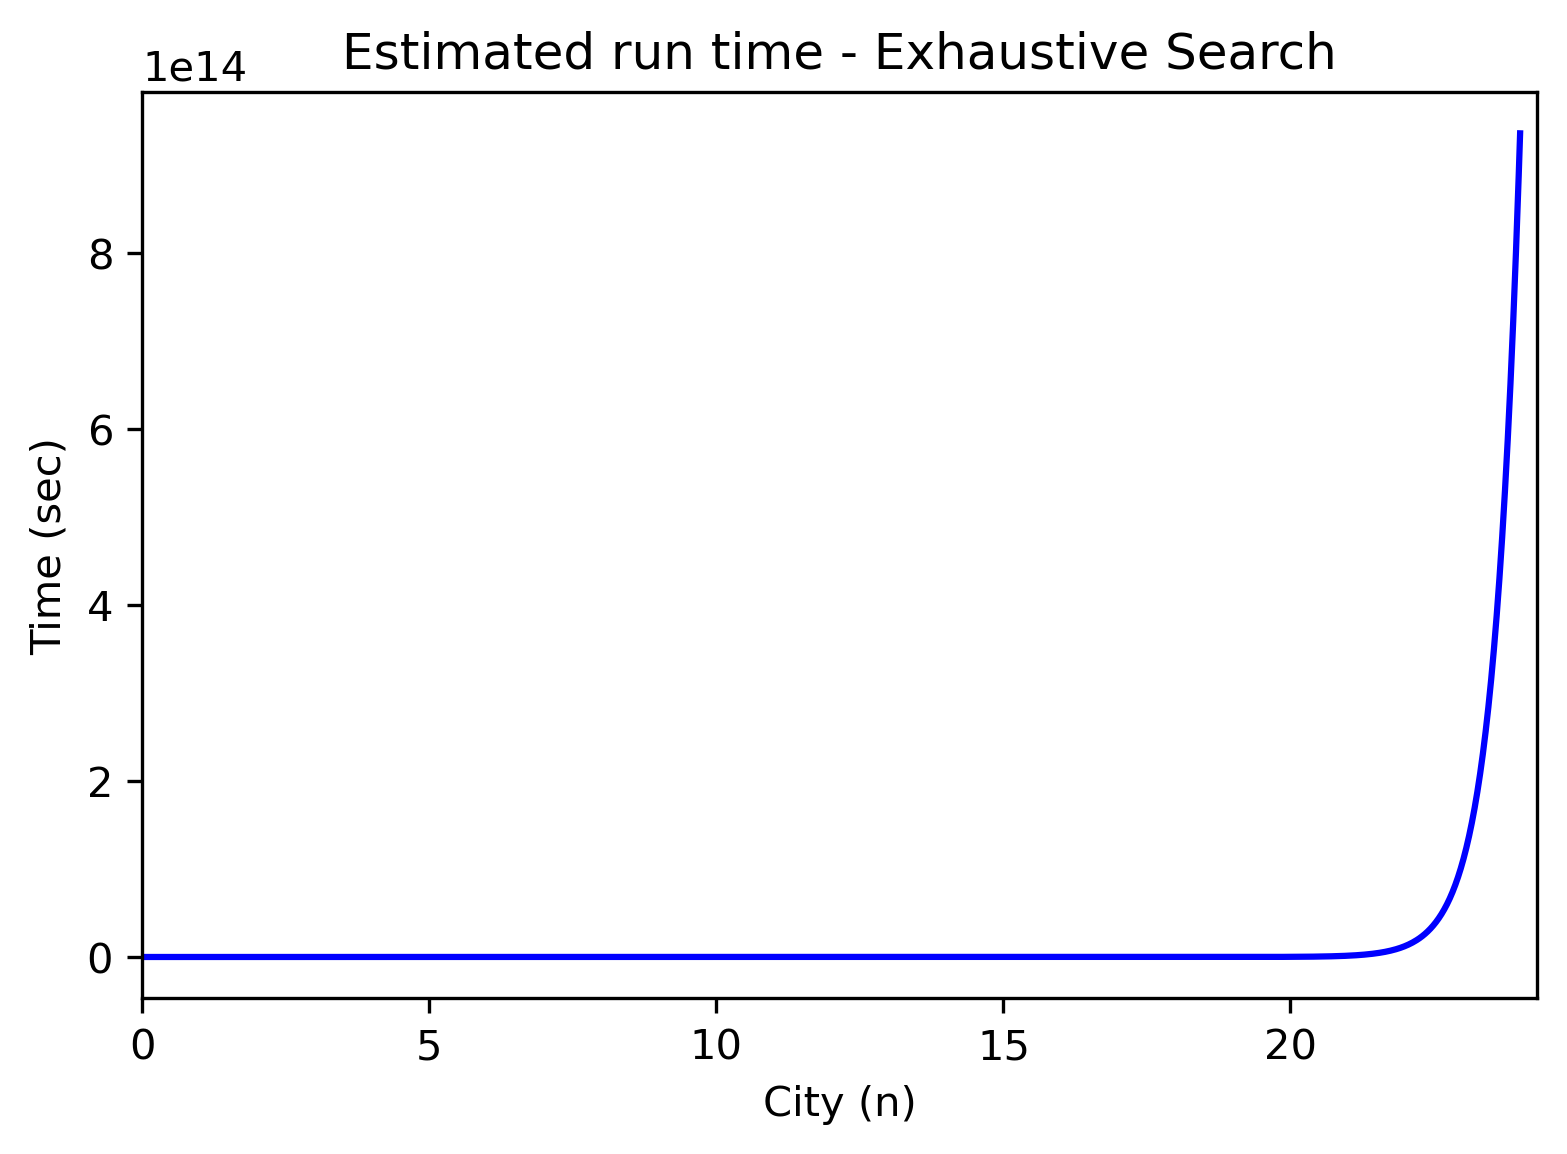
\includegraphics[width=6in, height=4in]{ExhaustiveSearch.png}}
\caption{Approximation of run time to find the best possible solution.}
\label{fig}
\end{figure}



Shortest tours for 6 and 10 cities:
\begin{figure}[H]
\centerline{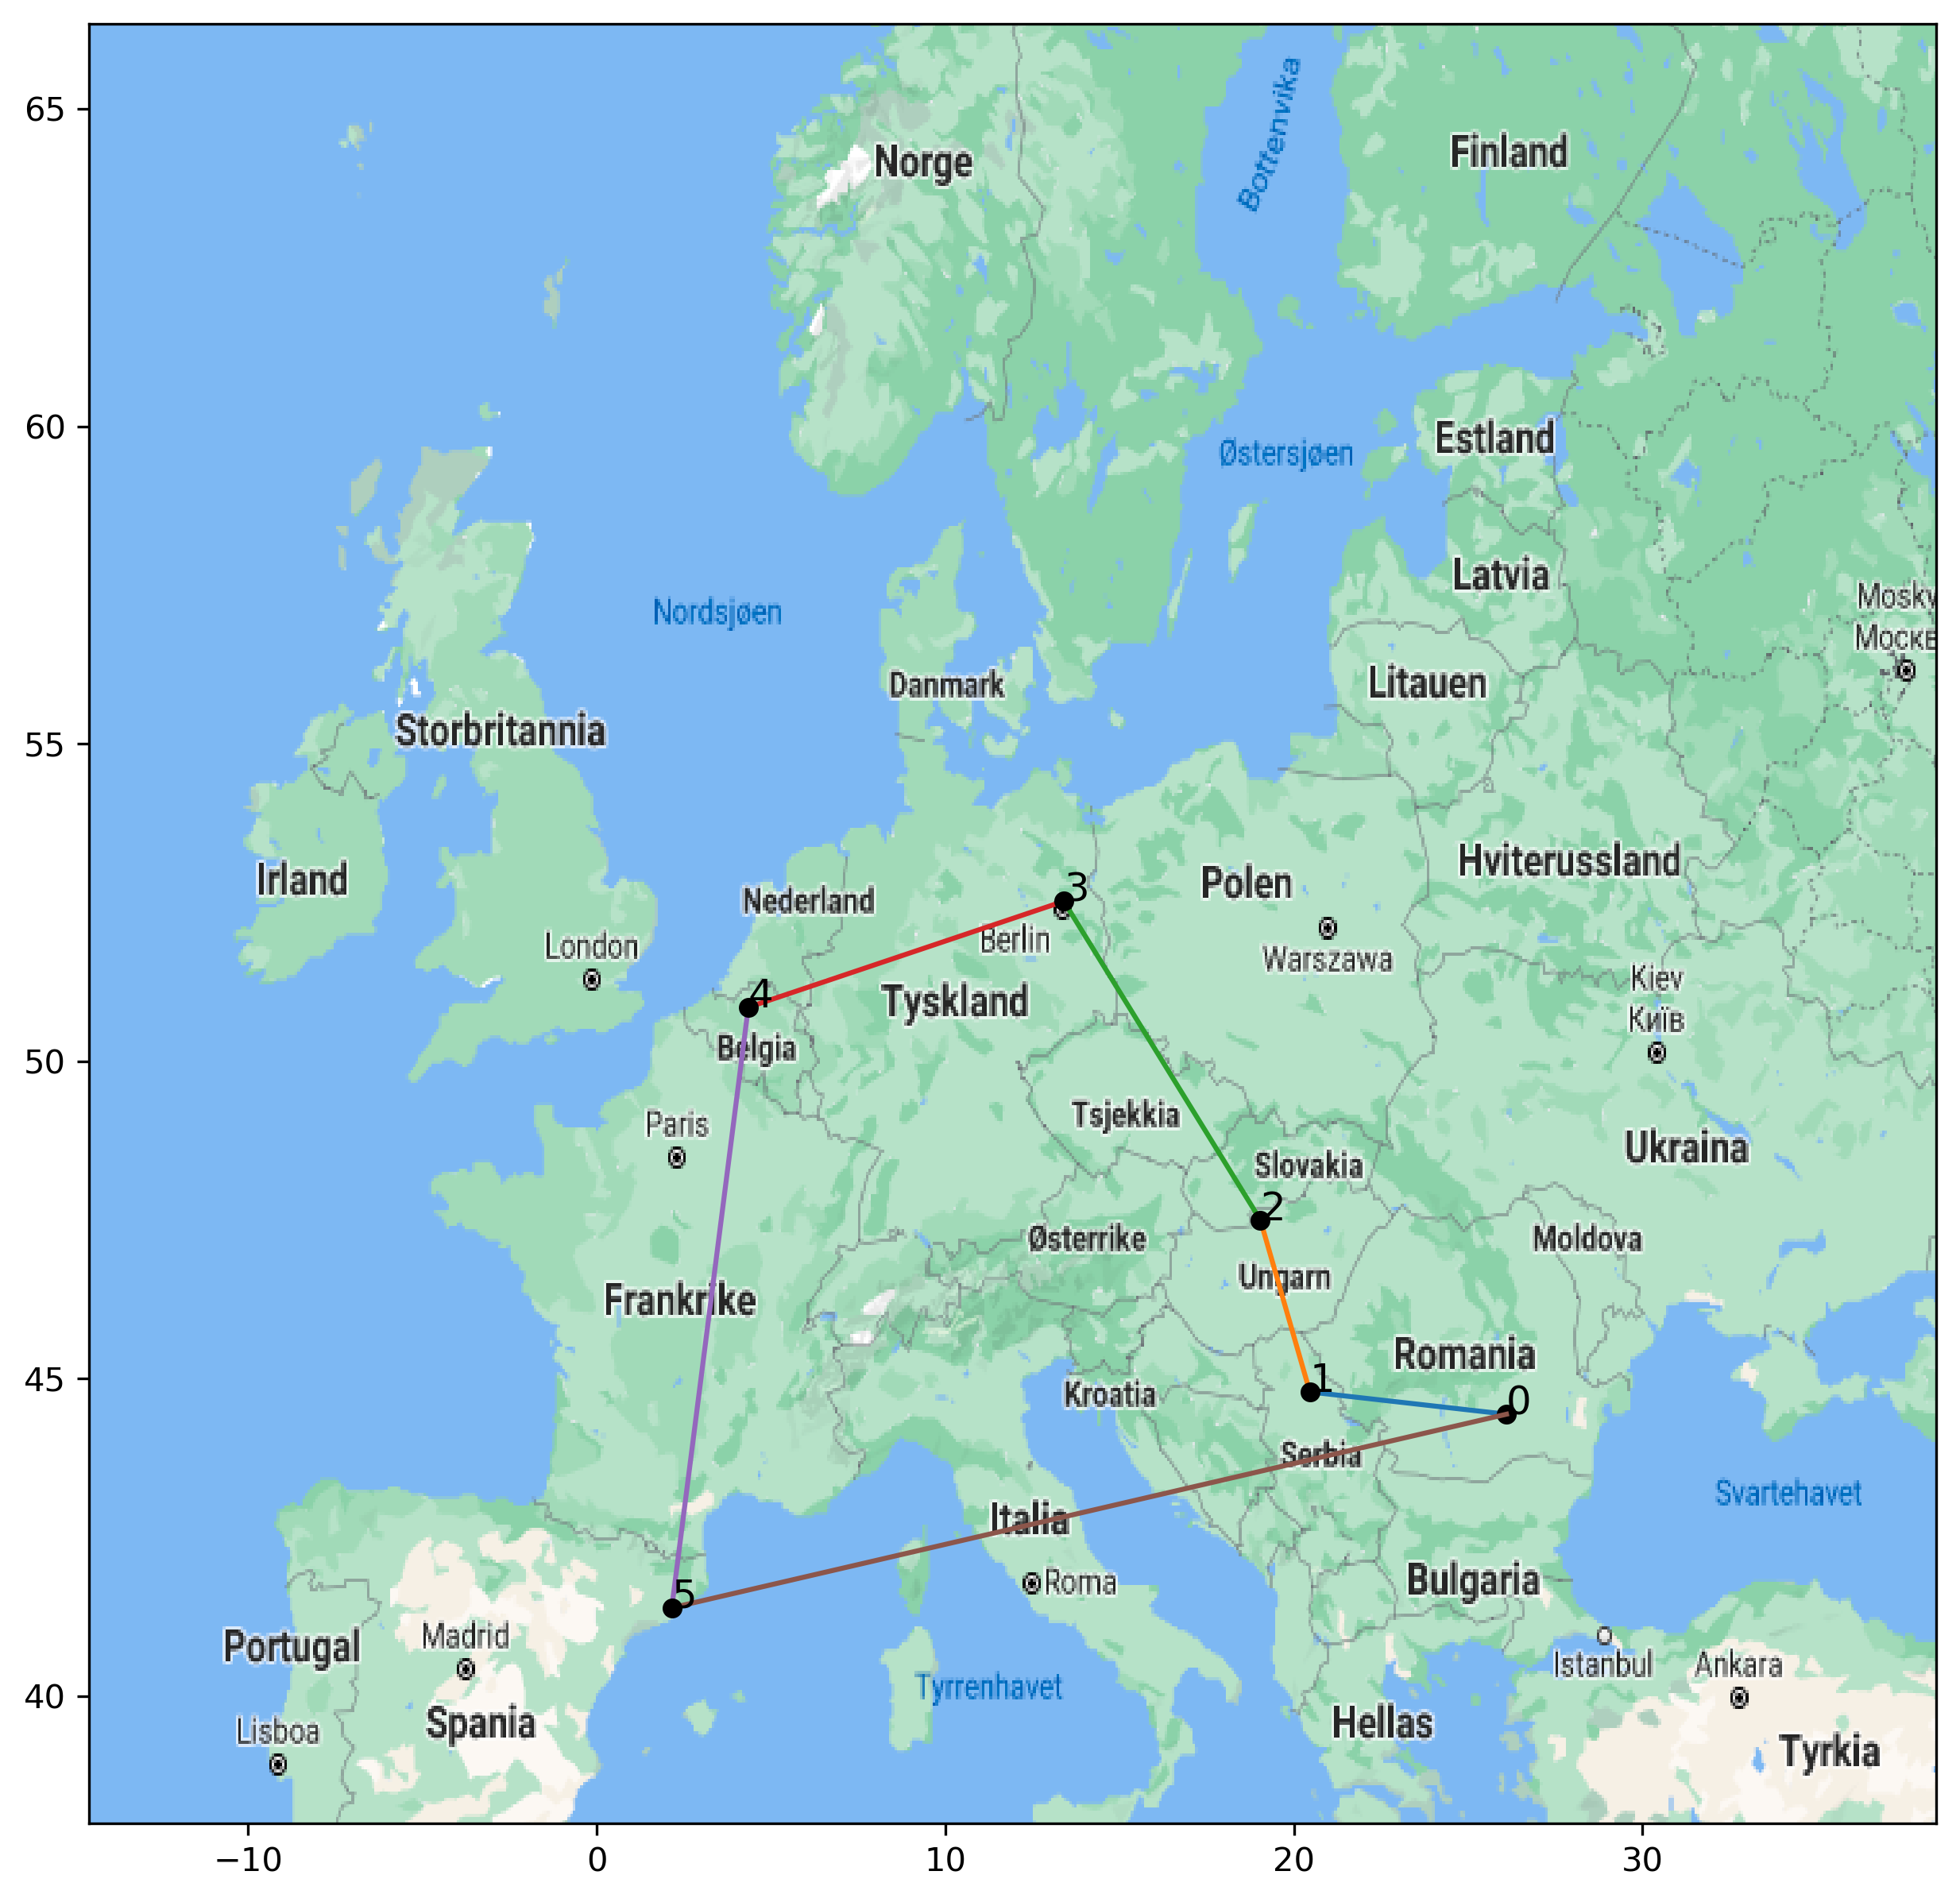
\includegraphics[width=6in, height=4in]{ExhaustiveSearchMap1.png}}
\caption{Shortest tour for 6 cities.}
\label{fig}
\end{figure}

\begin{figure}[H]
\centerline{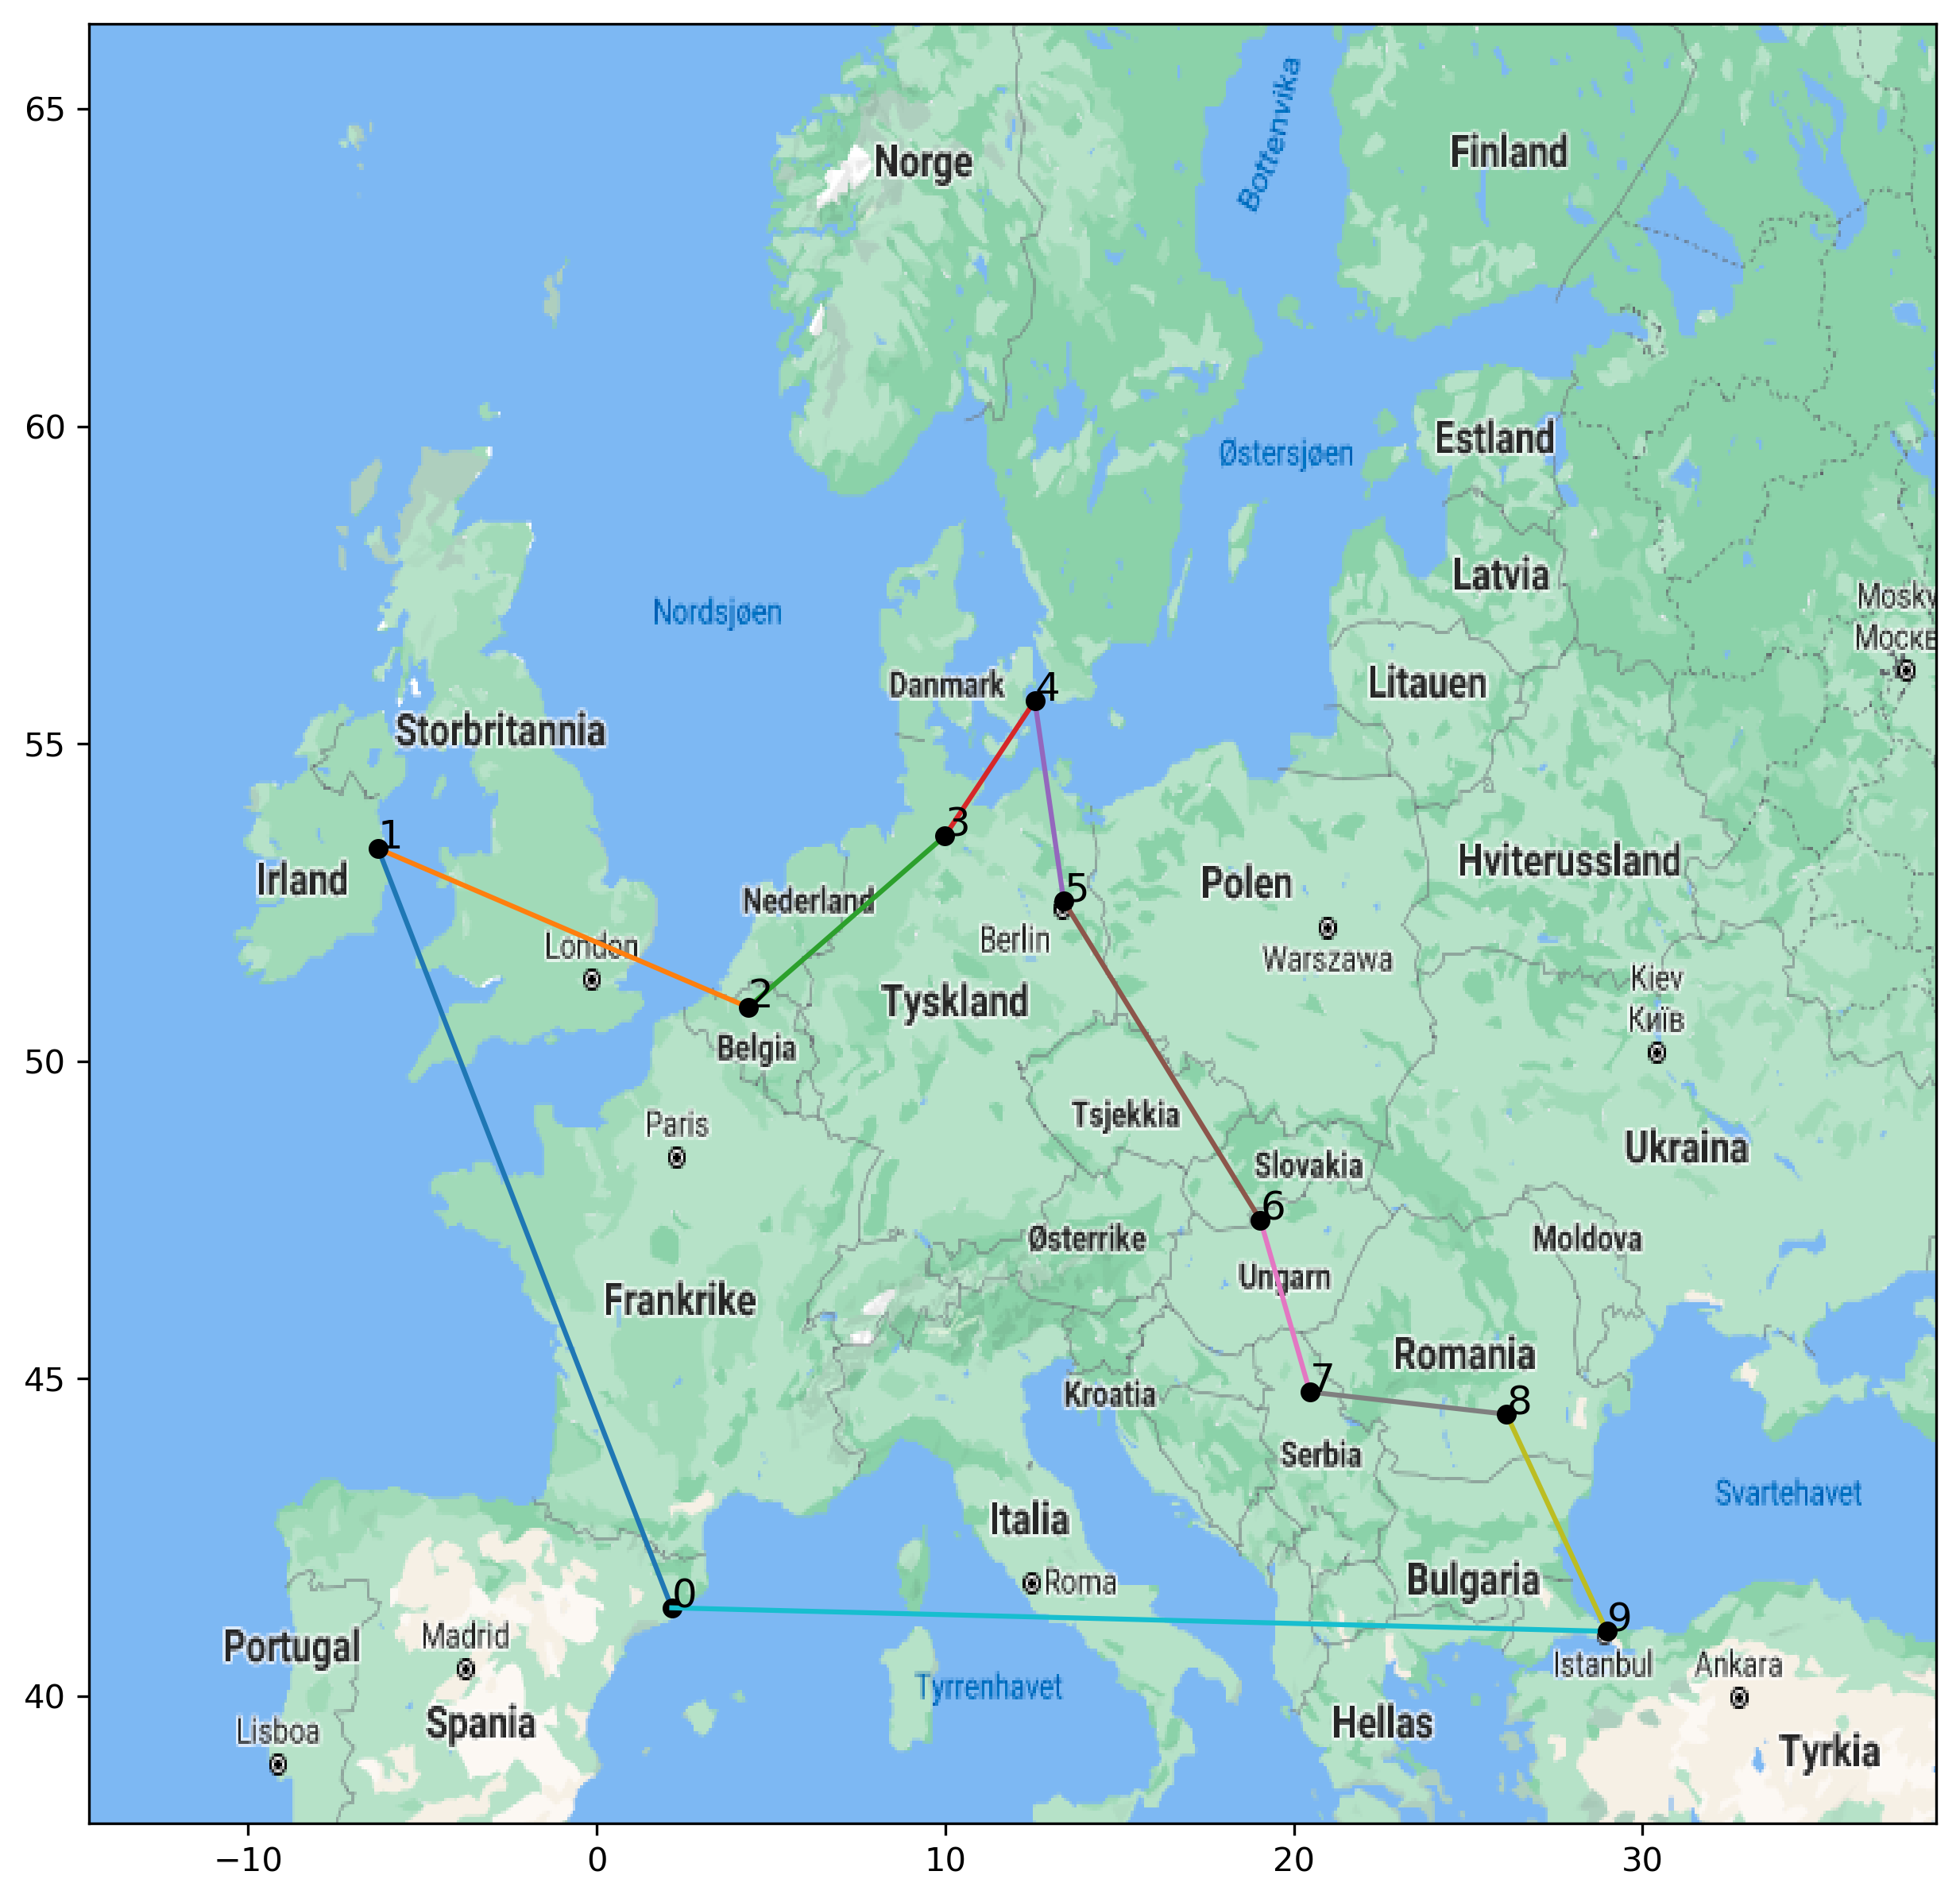
\includegraphics[width=6in, height=4in]{ExhaustiveSearchMap2.png}}
\caption{Shortest tour for 10 cities.}
\label{fig}
\end{figure}

\section{Hill Climbing }
The Hill Climbing algorithm is probabilistic in which the algorithm is searching random places in the landscape and tries to find the best solution by constantly climbing up in random directions. I used the swapping neighbors method. Where I choose two random genes in the parent and swapped them. If the mutation is better than the parent, we keep the mutation otherwise we use the parent. This is repeated number of times for each starting point in the landscape.  \\

Results for 10 cities: 20 runs and 1000 swaps per runs
\begin{center}
\begin{tabular}{c c}
 Number of runs & 20  \\ 
 Number of cities & 10  \\  
 Time used & 0.11073   \\  
 Best run & 5272.7   \\ 
Worst run & 6879.1   \\ 
Average & 6277.9   \\ 
 Standard deviation & 514.1   \\ 
\end{tabular}
\end{center}
Best sequence of cities: 'Barcelona', 'Dublin', 'Brussels', 'Hamburg', 'Copenhagen', 'Berlin', 'Budapest', 'Belgrade', 'Bucharest', 'Istanbul' \\ 
\begin{figure}[H]
\centerline{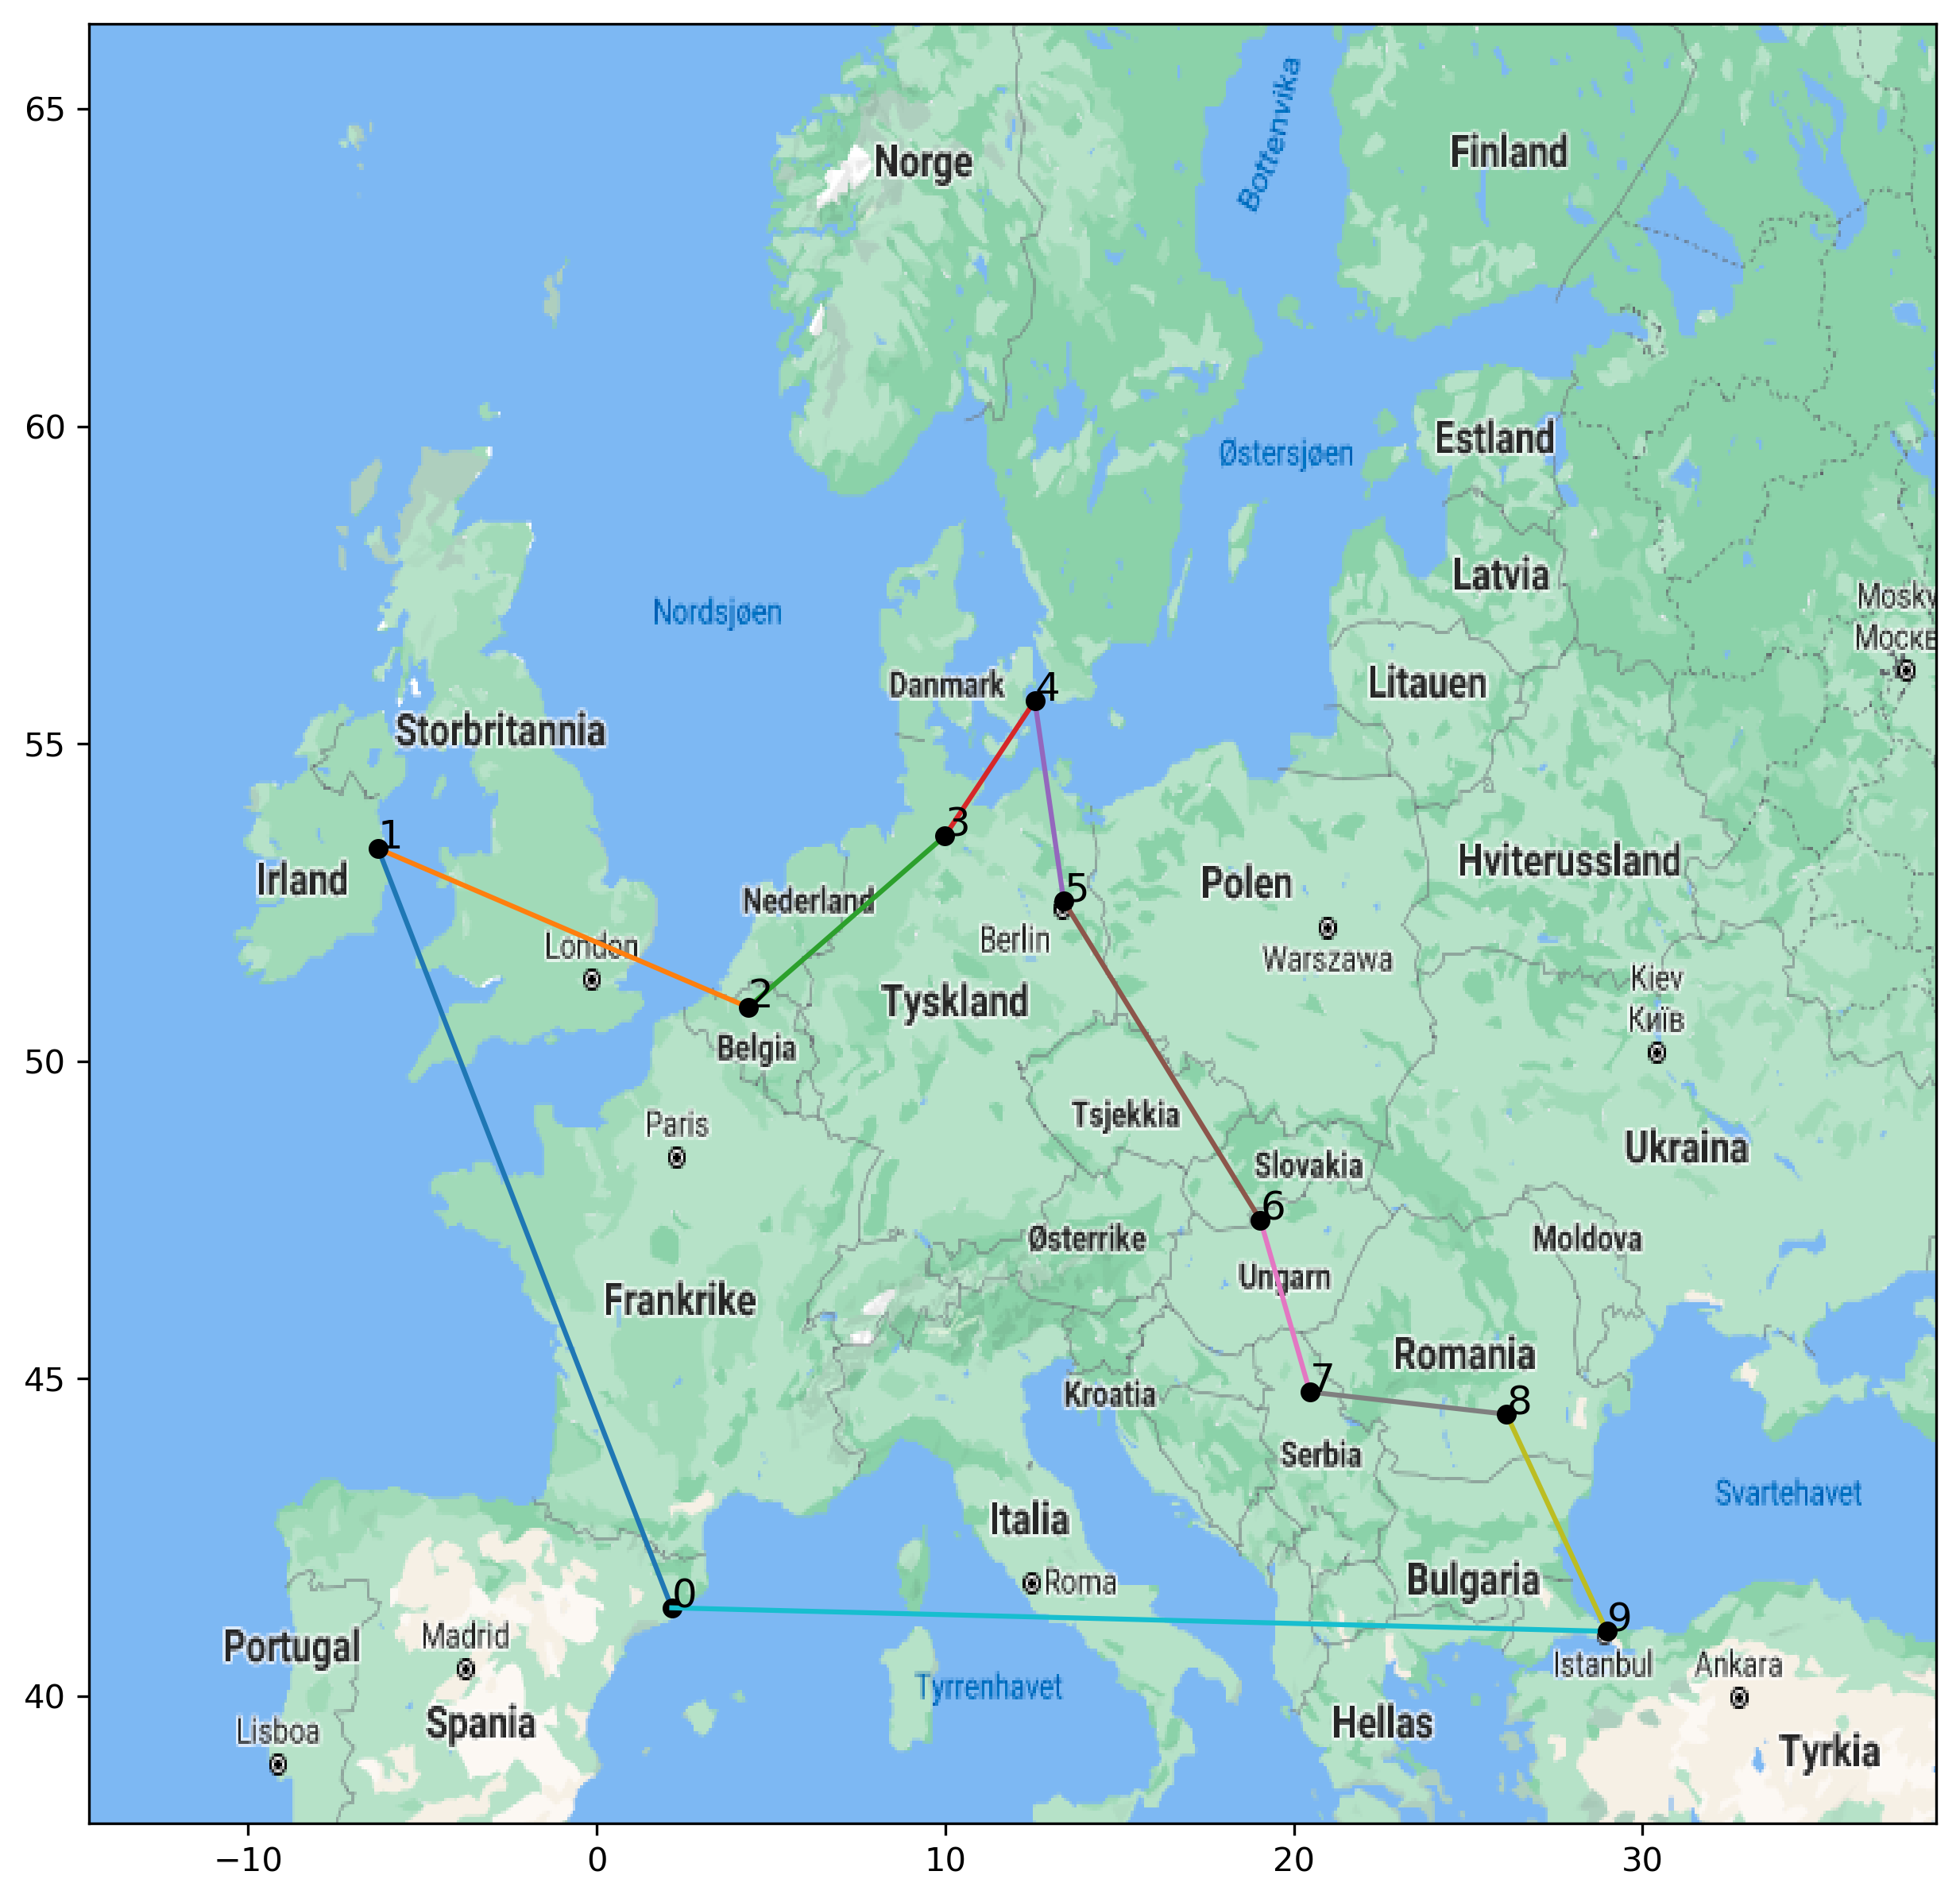
\includegraphics[width=6in, height=4in]{Hillclimber2.png}}
\caption{Map of 10 cities.}
\label{fig}
\end{figure}

Results for 24 cities: 20 runs and 1000 swaps per runs
\begin{center}
\begin{tabular}{ c c}
 Number of runs & 20  \\ 
 Number of cities & 24  \\  
 Time used & 0.1855   \\  
 Best run & 12721.4   \\ 
Worst run & 15404.2  \\ 
Average & 13837.9   \\ 
 Standard deviation & 701.5   \\ 
\end{tabular}
\end{center}
Time to find global solution for 24 cities using a simple hill climbing algorithm:  87.78  seconds.\\

Best sequence of cities: 'Madrid', 'Barcelona', 'Paris', 'Hamburg', 'Copenhagen', 'Berlin', 'Warsaw', 'Stockholm', 'Saint Petersburg', 'Moscow', 'Kiev', 'Bucharest', 'Istanbul', 'Sofia', 'Belgrade', 'Budapest', 'Rome', 'Milan', 'Vienna', 'Prague', 'Munich', 'Brussels', 'London', 'Dublin' \\ 

\begin{figure}[H]
\centerline{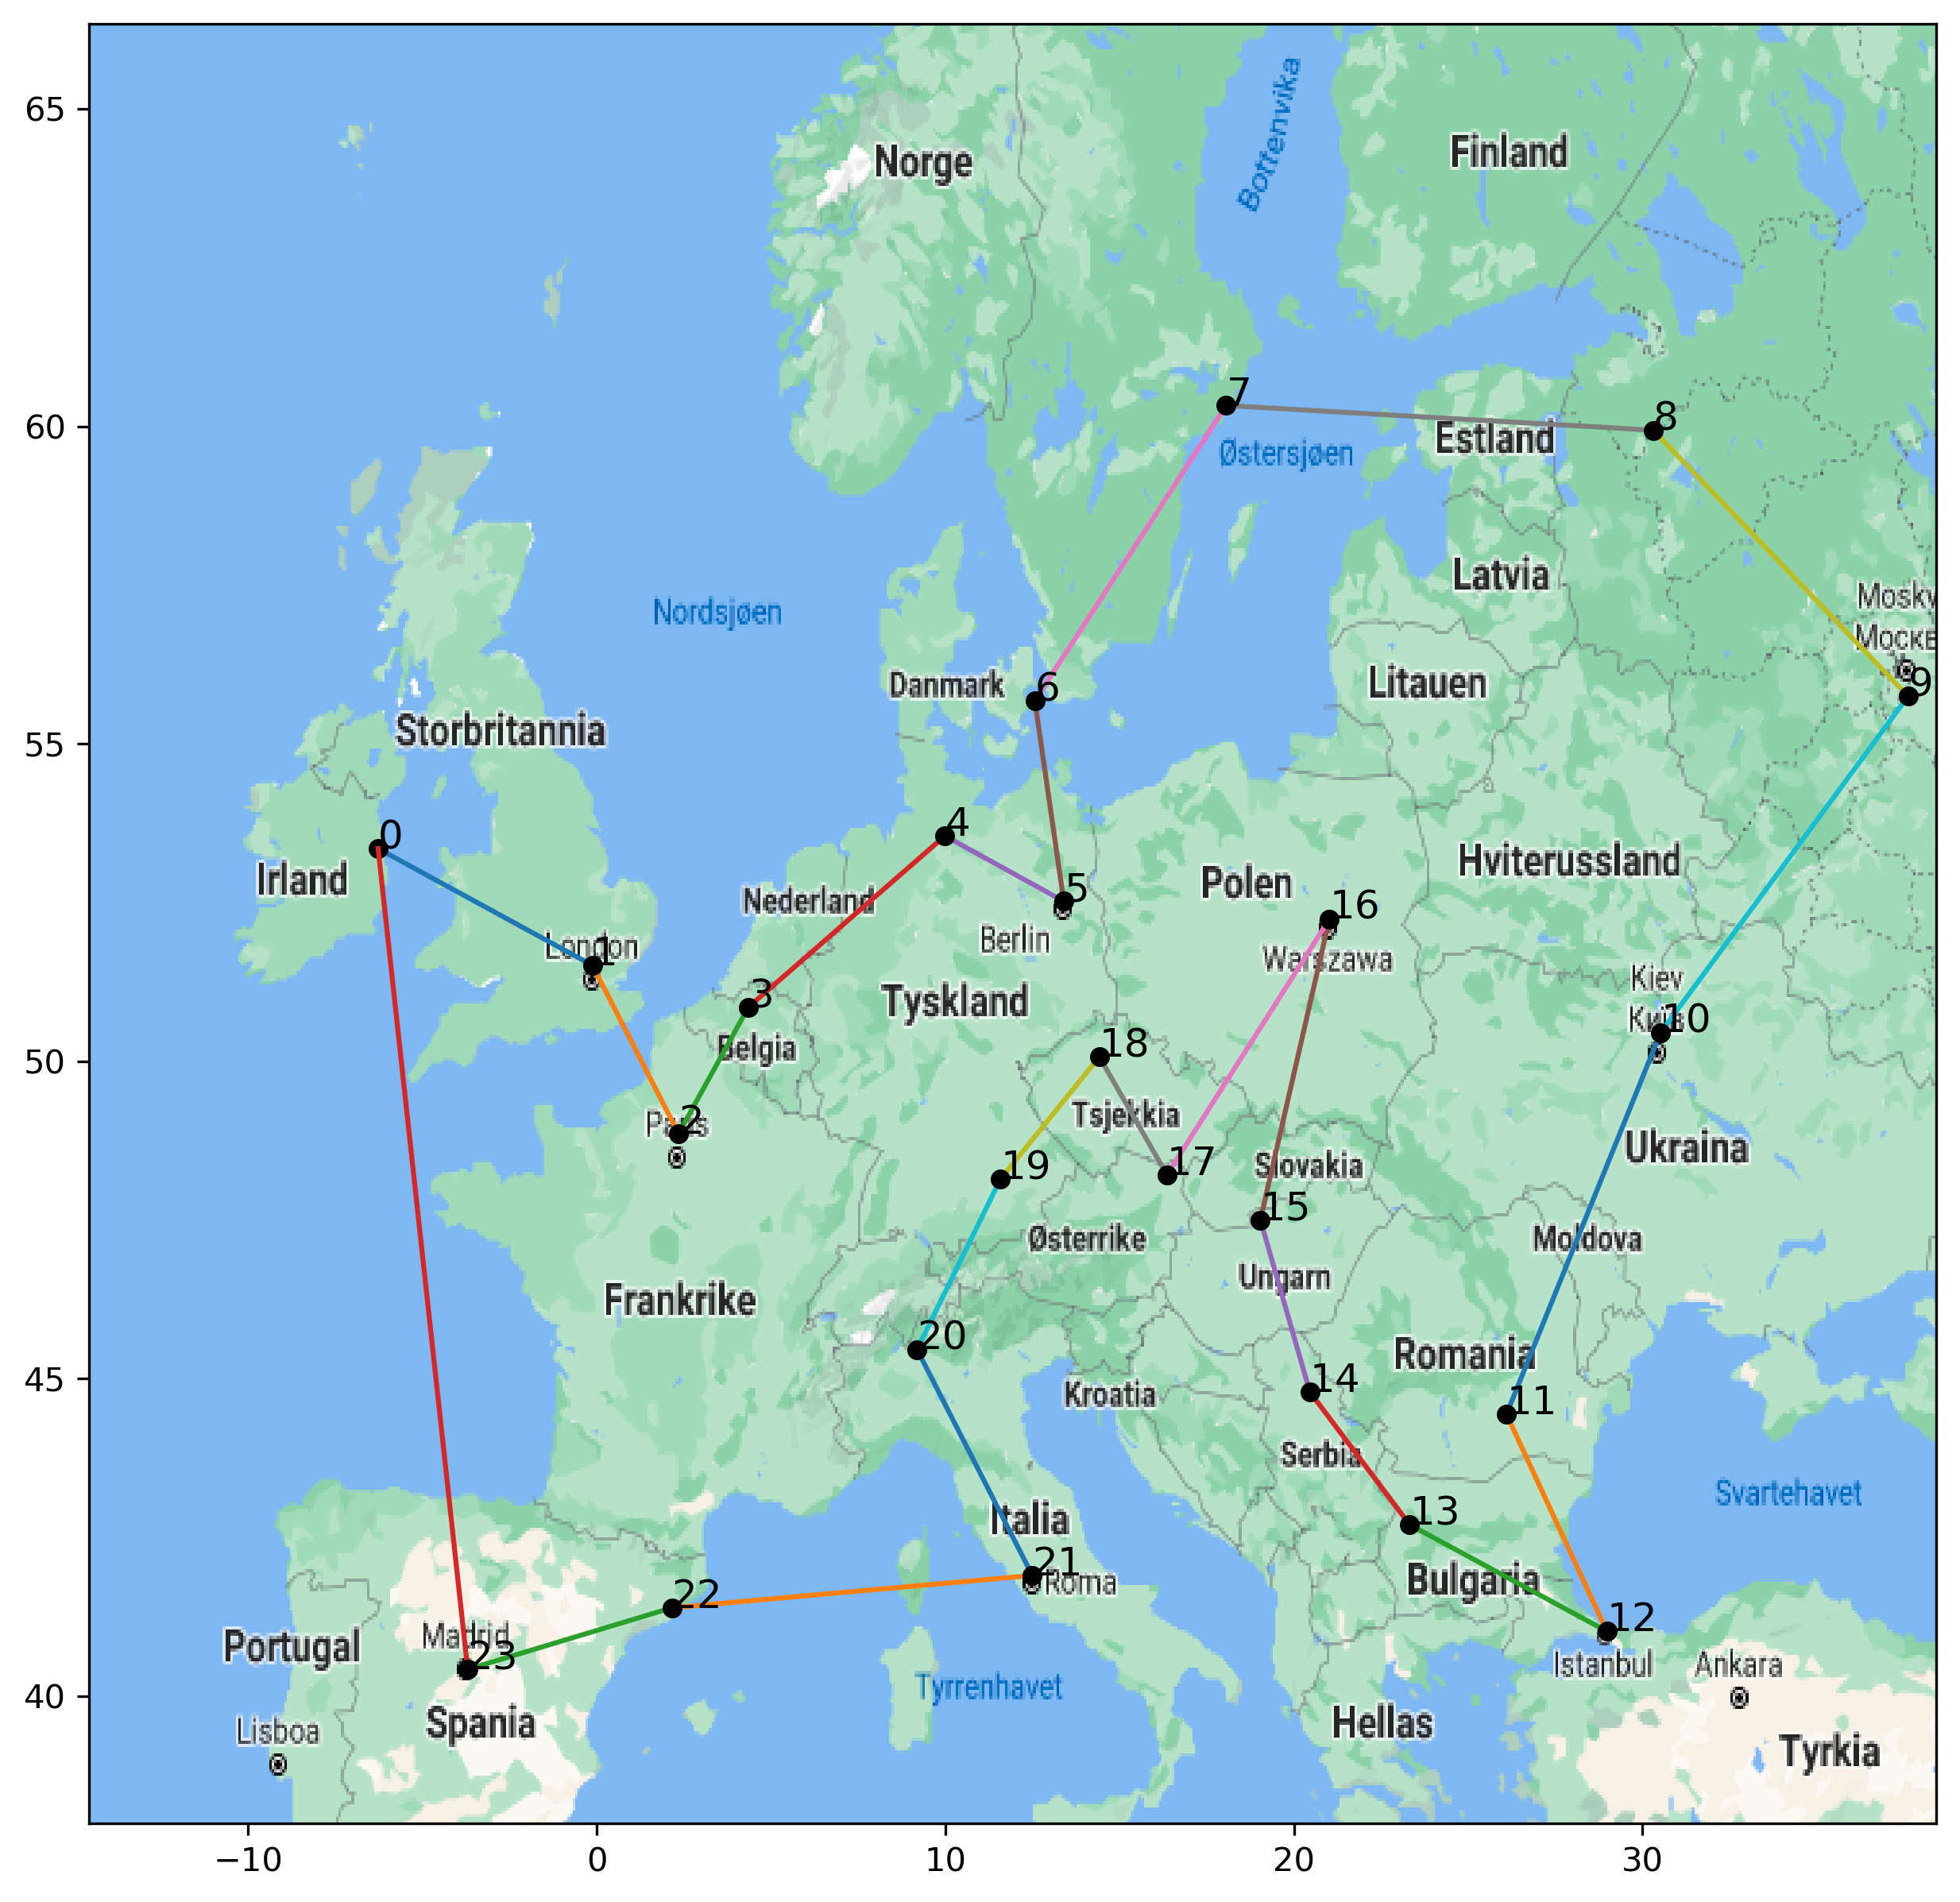
\includegraphics[width=6in, height=4in]{Hillclimber1.png}}
\caption{Map of 24 cities.}
\label{fig}
\end{figure}

As excepted the hill climber is much faster than the exhaustive search. The hill climbing algorithm is really good at finding a local optima, however for larger number of cities its run time becomes large since there are many local minimums and the algorithm has to do more exploration and therefore it becomes harder to find the global minimum, as can be seen in the graph below. The hill climbing algorithm found the best solution for 10 cities, however for 24 cities it is far from a global solution.

\begin{figure}[H]
\centerline{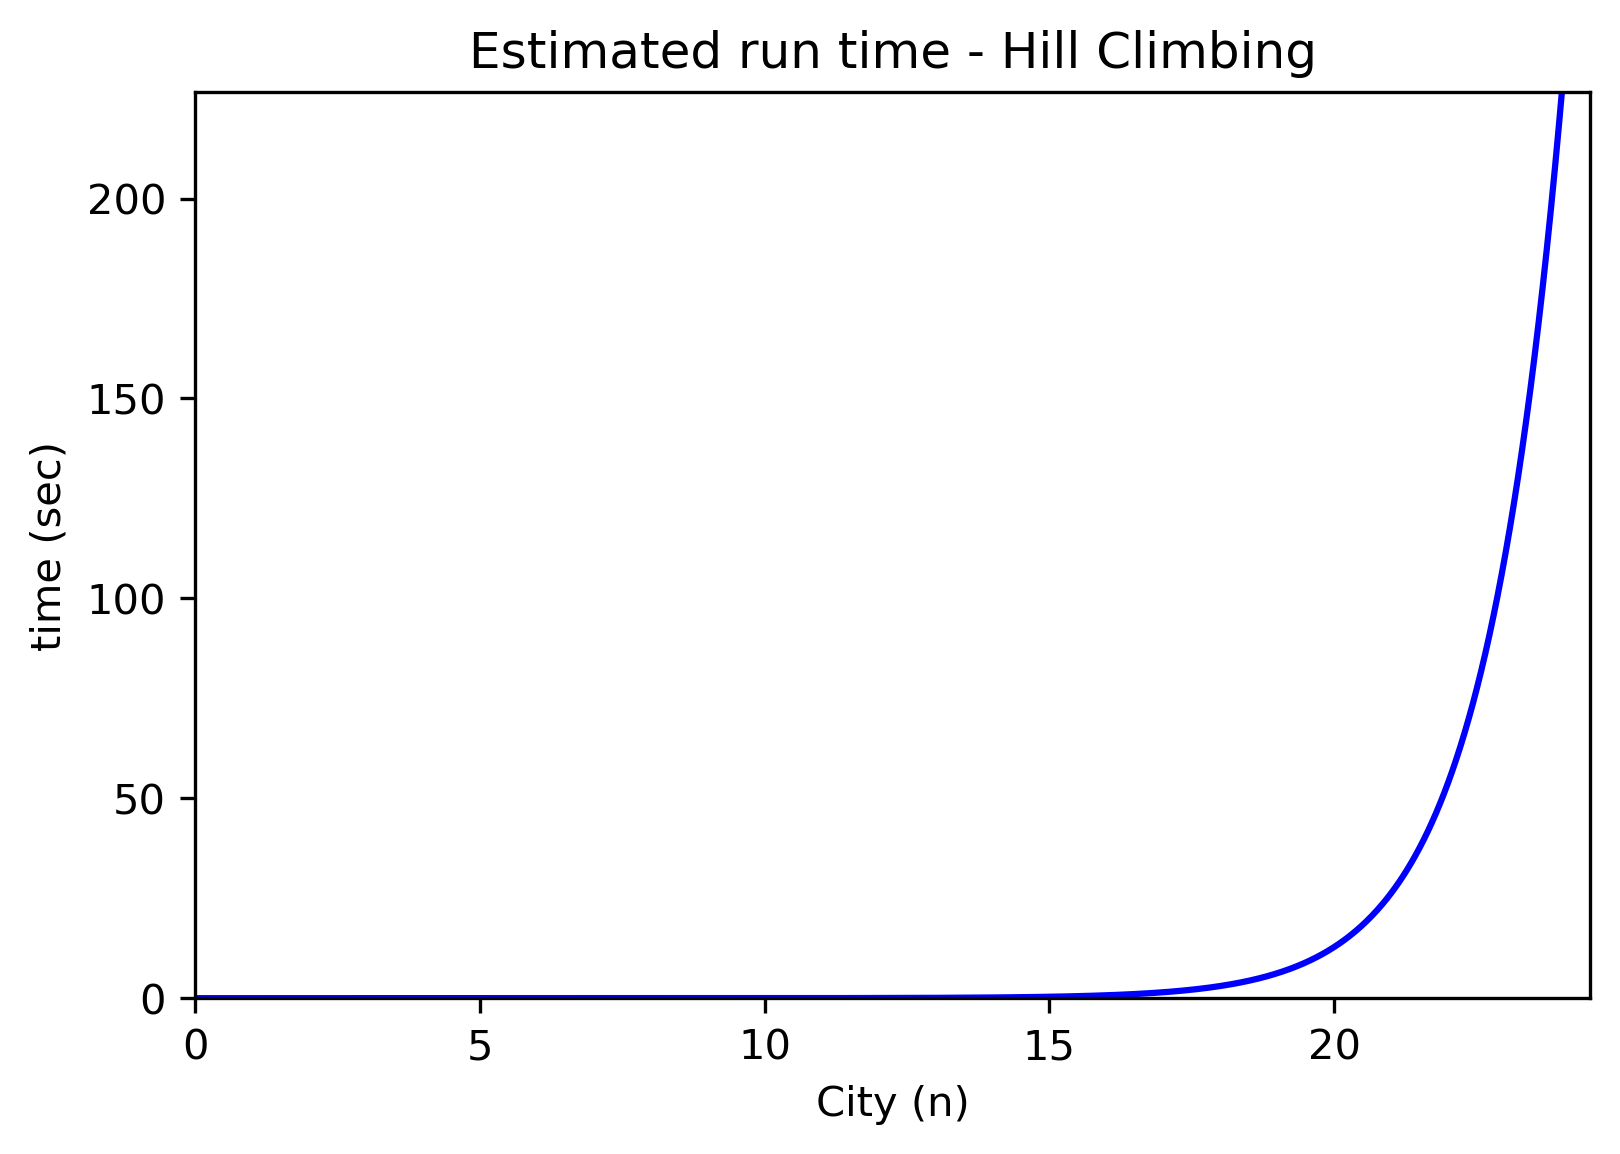
\includegraphics[width=6in, height=4in]{HillClimber-fit.png}}
\caption{Time required to find the best solution for a given number of cities.}
\label{fig}
\end{figure}

\section{Genetic Algorithm}
In the genetic algorithm, we start by selecting a random number population based on a number of genes (cities), the population then goes through re-combinations and mutations. After they are mated, population seize is increased to dobbel. In my algorithm the population remains constant, therefore the parents and their offspring are competing and are selected based on the best fitness values. Only half of the current population will survive for the next generation. For example 2 parents will have 2 children or the parents might mutate to two new individuals. After all the population have gone through either mutation or recombination, half of this will be selected in the next generation. This will continue until the last generation.\\ 

I used a mutation rate of 0.01, mutation rate higher showed worst results. I used 4 mutation operators with inversion mutation giving the best result, and therefore highest probability of being chosen. After that insert mutation was the next best mutation operator. Insert and swap mutation showed to be not that effective. For the recombination operators, order crossover gave best results together with partially mapped crossover, and cycle crossover was not that good of a choice.\\

Results for 3 different populations and 20 generations:\\
\begin{center}
\begin{tabular}{ c c}
 Population & 10  \\ 
 Number of runs & 20  \\ 
 Number of cities & 10  \\  
Tours inspected & 200  \\
 Time used & 0.00399   \\  
 Best run & 5914.4  \\ 
Worst run &  8693.1  \\ 
Average & 7707.9   \\ 
 Standard deviation & 811.6   \\ 


\end{tabular}
\end{center}
Best sequence of cities: ''Budapest', 'Copenhagen', 'Berlin', 'Hamburg', 'Brussels', 'Dublin', 'Barcelona', 'Belgrade', 'Bucharest', 'Istanbul'' \\ 

\begin{figure}[H]
\centerline{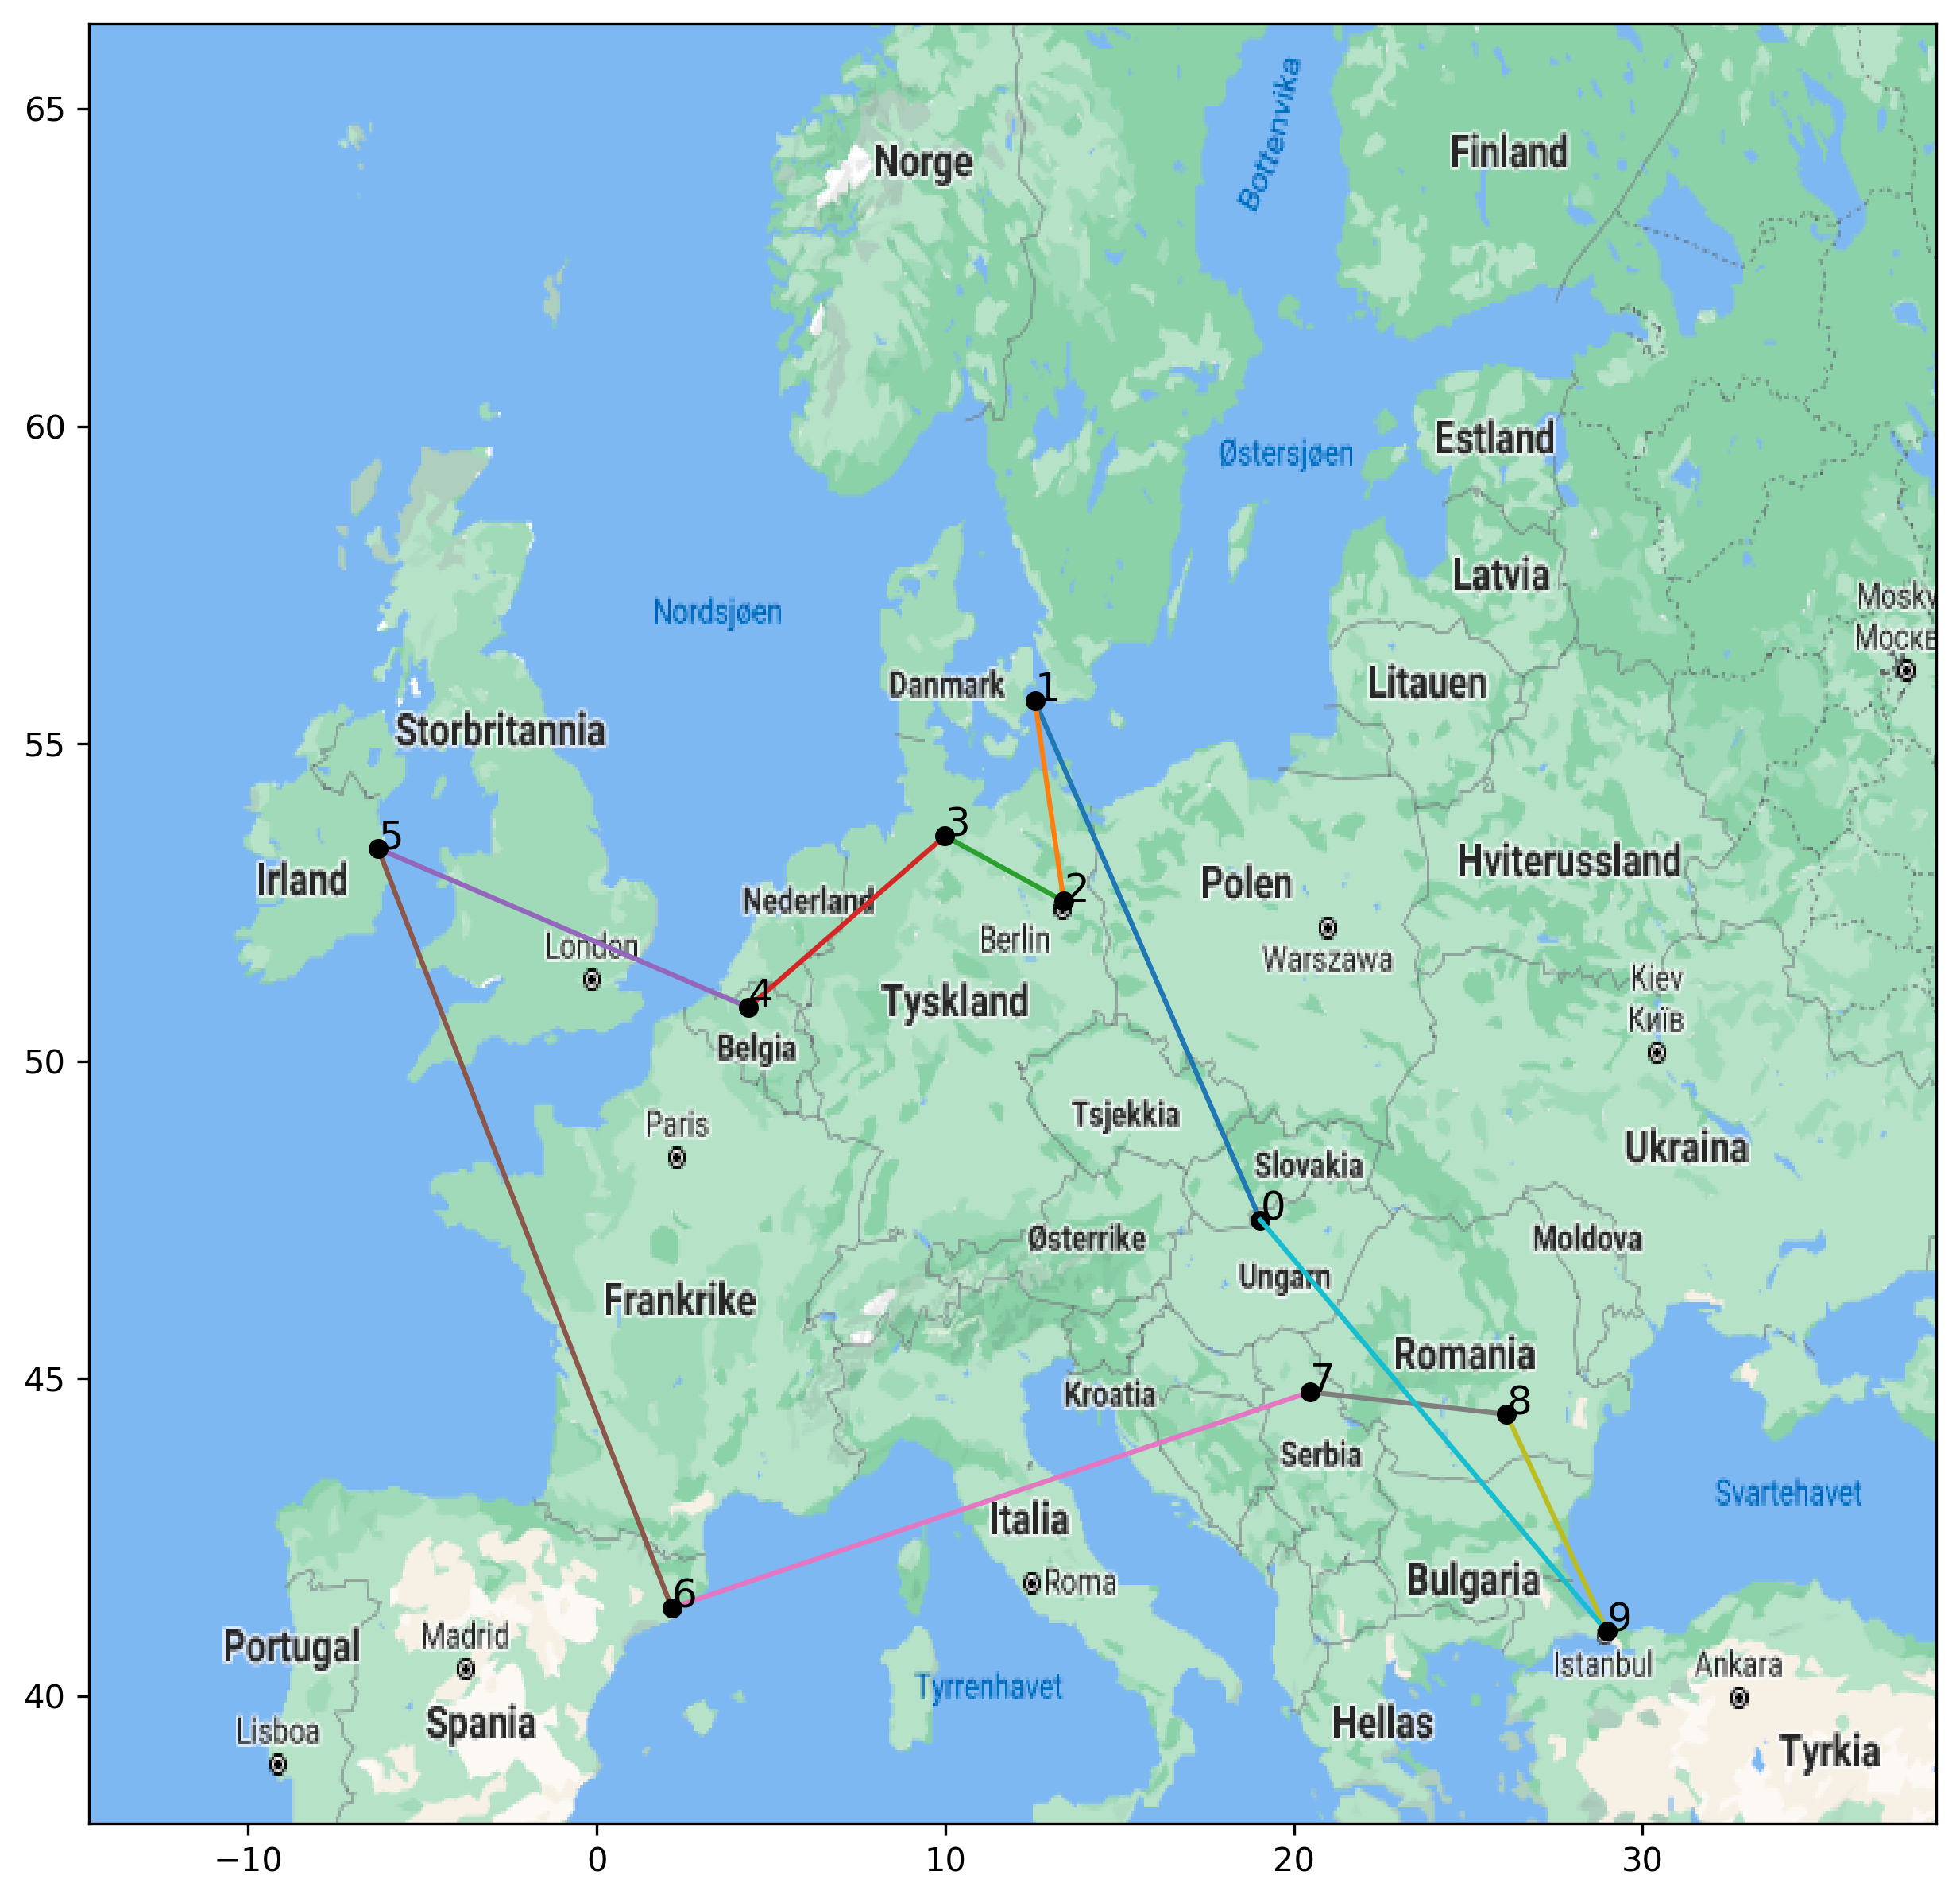
\includegraphics[width=6in, height=4in]{geneticMap1.png}}
\caption{City=10, population=10, generation=20.}
\label{fig}
\end{figure}

\begin{center}
\begin{tabular}{ c c}
 Population & 100  \\ 
 Number of runs & 20  \\ 
 Number of cities & 10  \\  
Tours inspected & 2000  \\
 Time used & 0.04089   \\  
 Best run & 5755.0  \\ 
Worst run & 9695.7  \\ 
Average & 7928.7   \\ 
 Standard deviation & 767.8   \\ 
\end{tabular}
\end{center}


Best sequence of cities: 'Istanbul', 'Bucharest', 'Belgrade', 'Budapest', 'Berlin', 'Hamburg', 'Copenhagen', 'Brussels', 'Dublin', 'Barcelona' \\ 
\begin{figure}[H]
\centerline{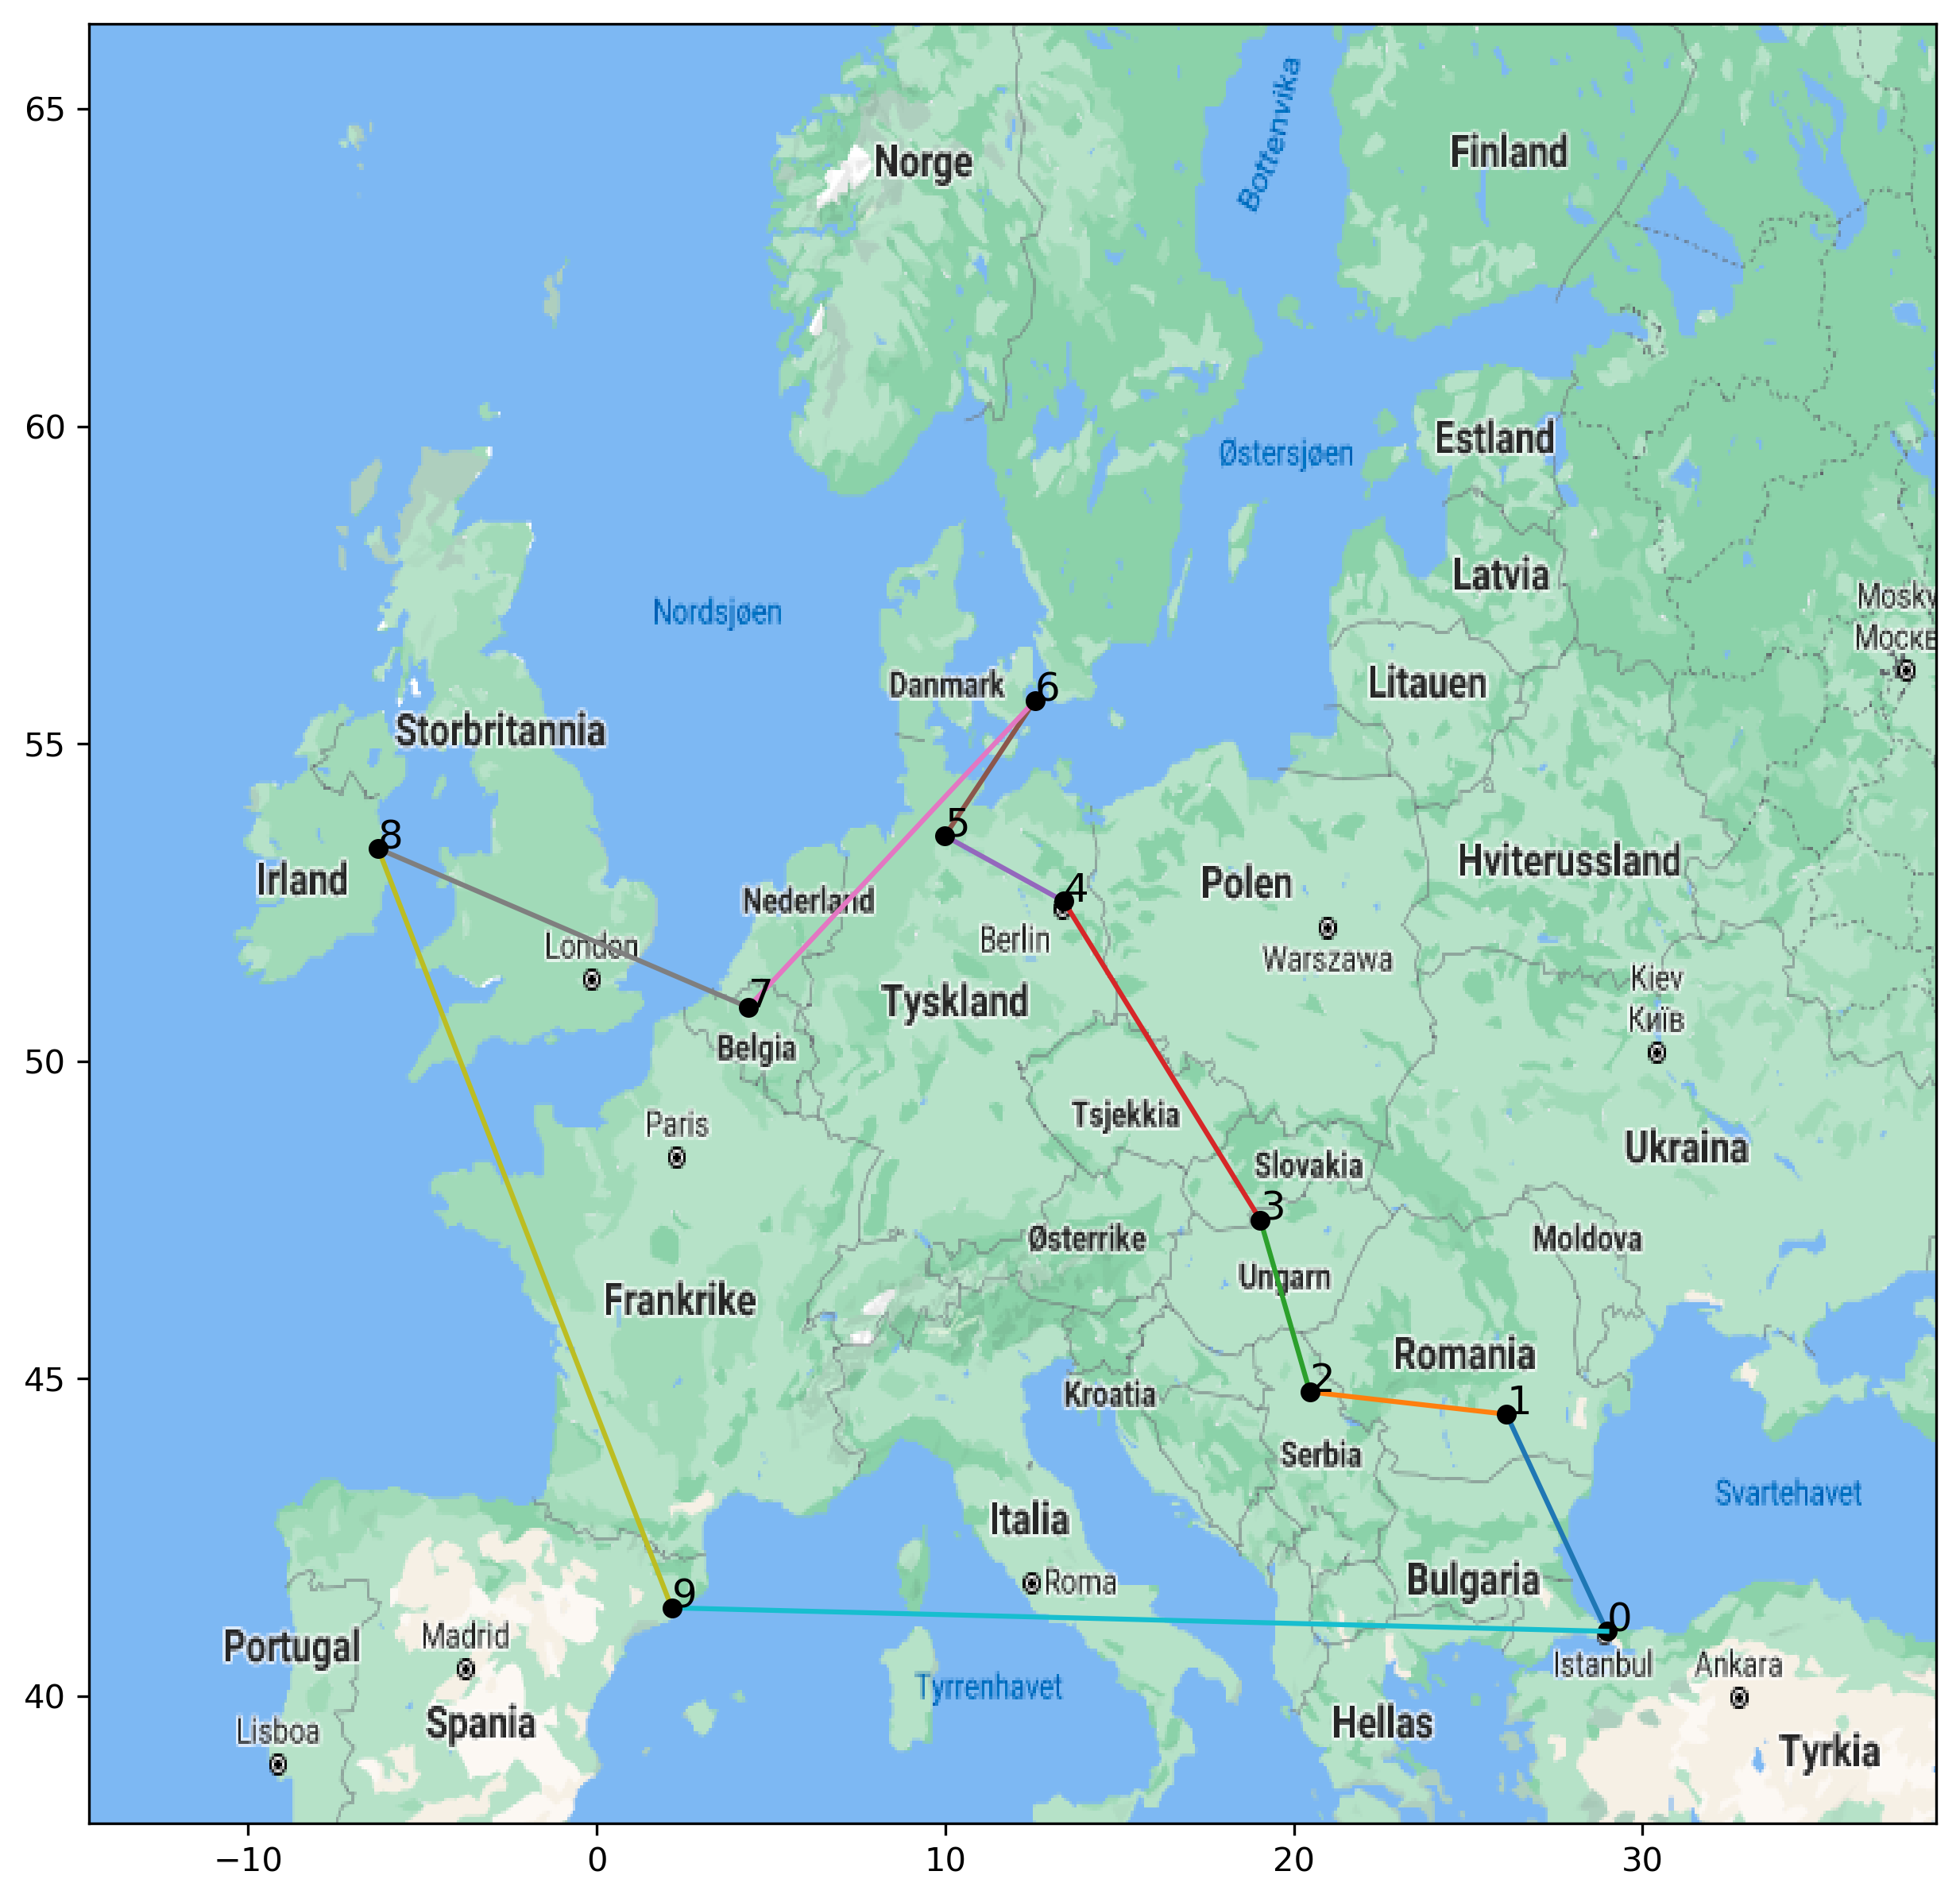
\includegraphics[width=6in, height=4in]{geneticMap2.png}}
\caption{City=10, population=100, generation=20.}
\label{fig}
\end{figure}

\begin{center}
\begin{tabular}{ c c}
 Population & 1000  \\ 
 Number of runs & 20  \\ 
 Number of cities & 10  \\  
Tours inspected & 20000  \\
 Time used & 0.38494   \\  
 Best run & 5272.7  \\ 
Worst run &  10386.0 \\ 
Average & 7860.1  \\ 
 Standard deviation & 786.3 \\ 


\end{tabular}
\end{center}
Best sequence of cities: 'Barcelona', 'Dublin', 'Brussels', 'Hamburg', 'Berlin', 'Copenhagen', 'Budapest', 'Belgrade', 'Bucharest', 'Istanbul'\\ 
\begin{figure}[H]
\centerline{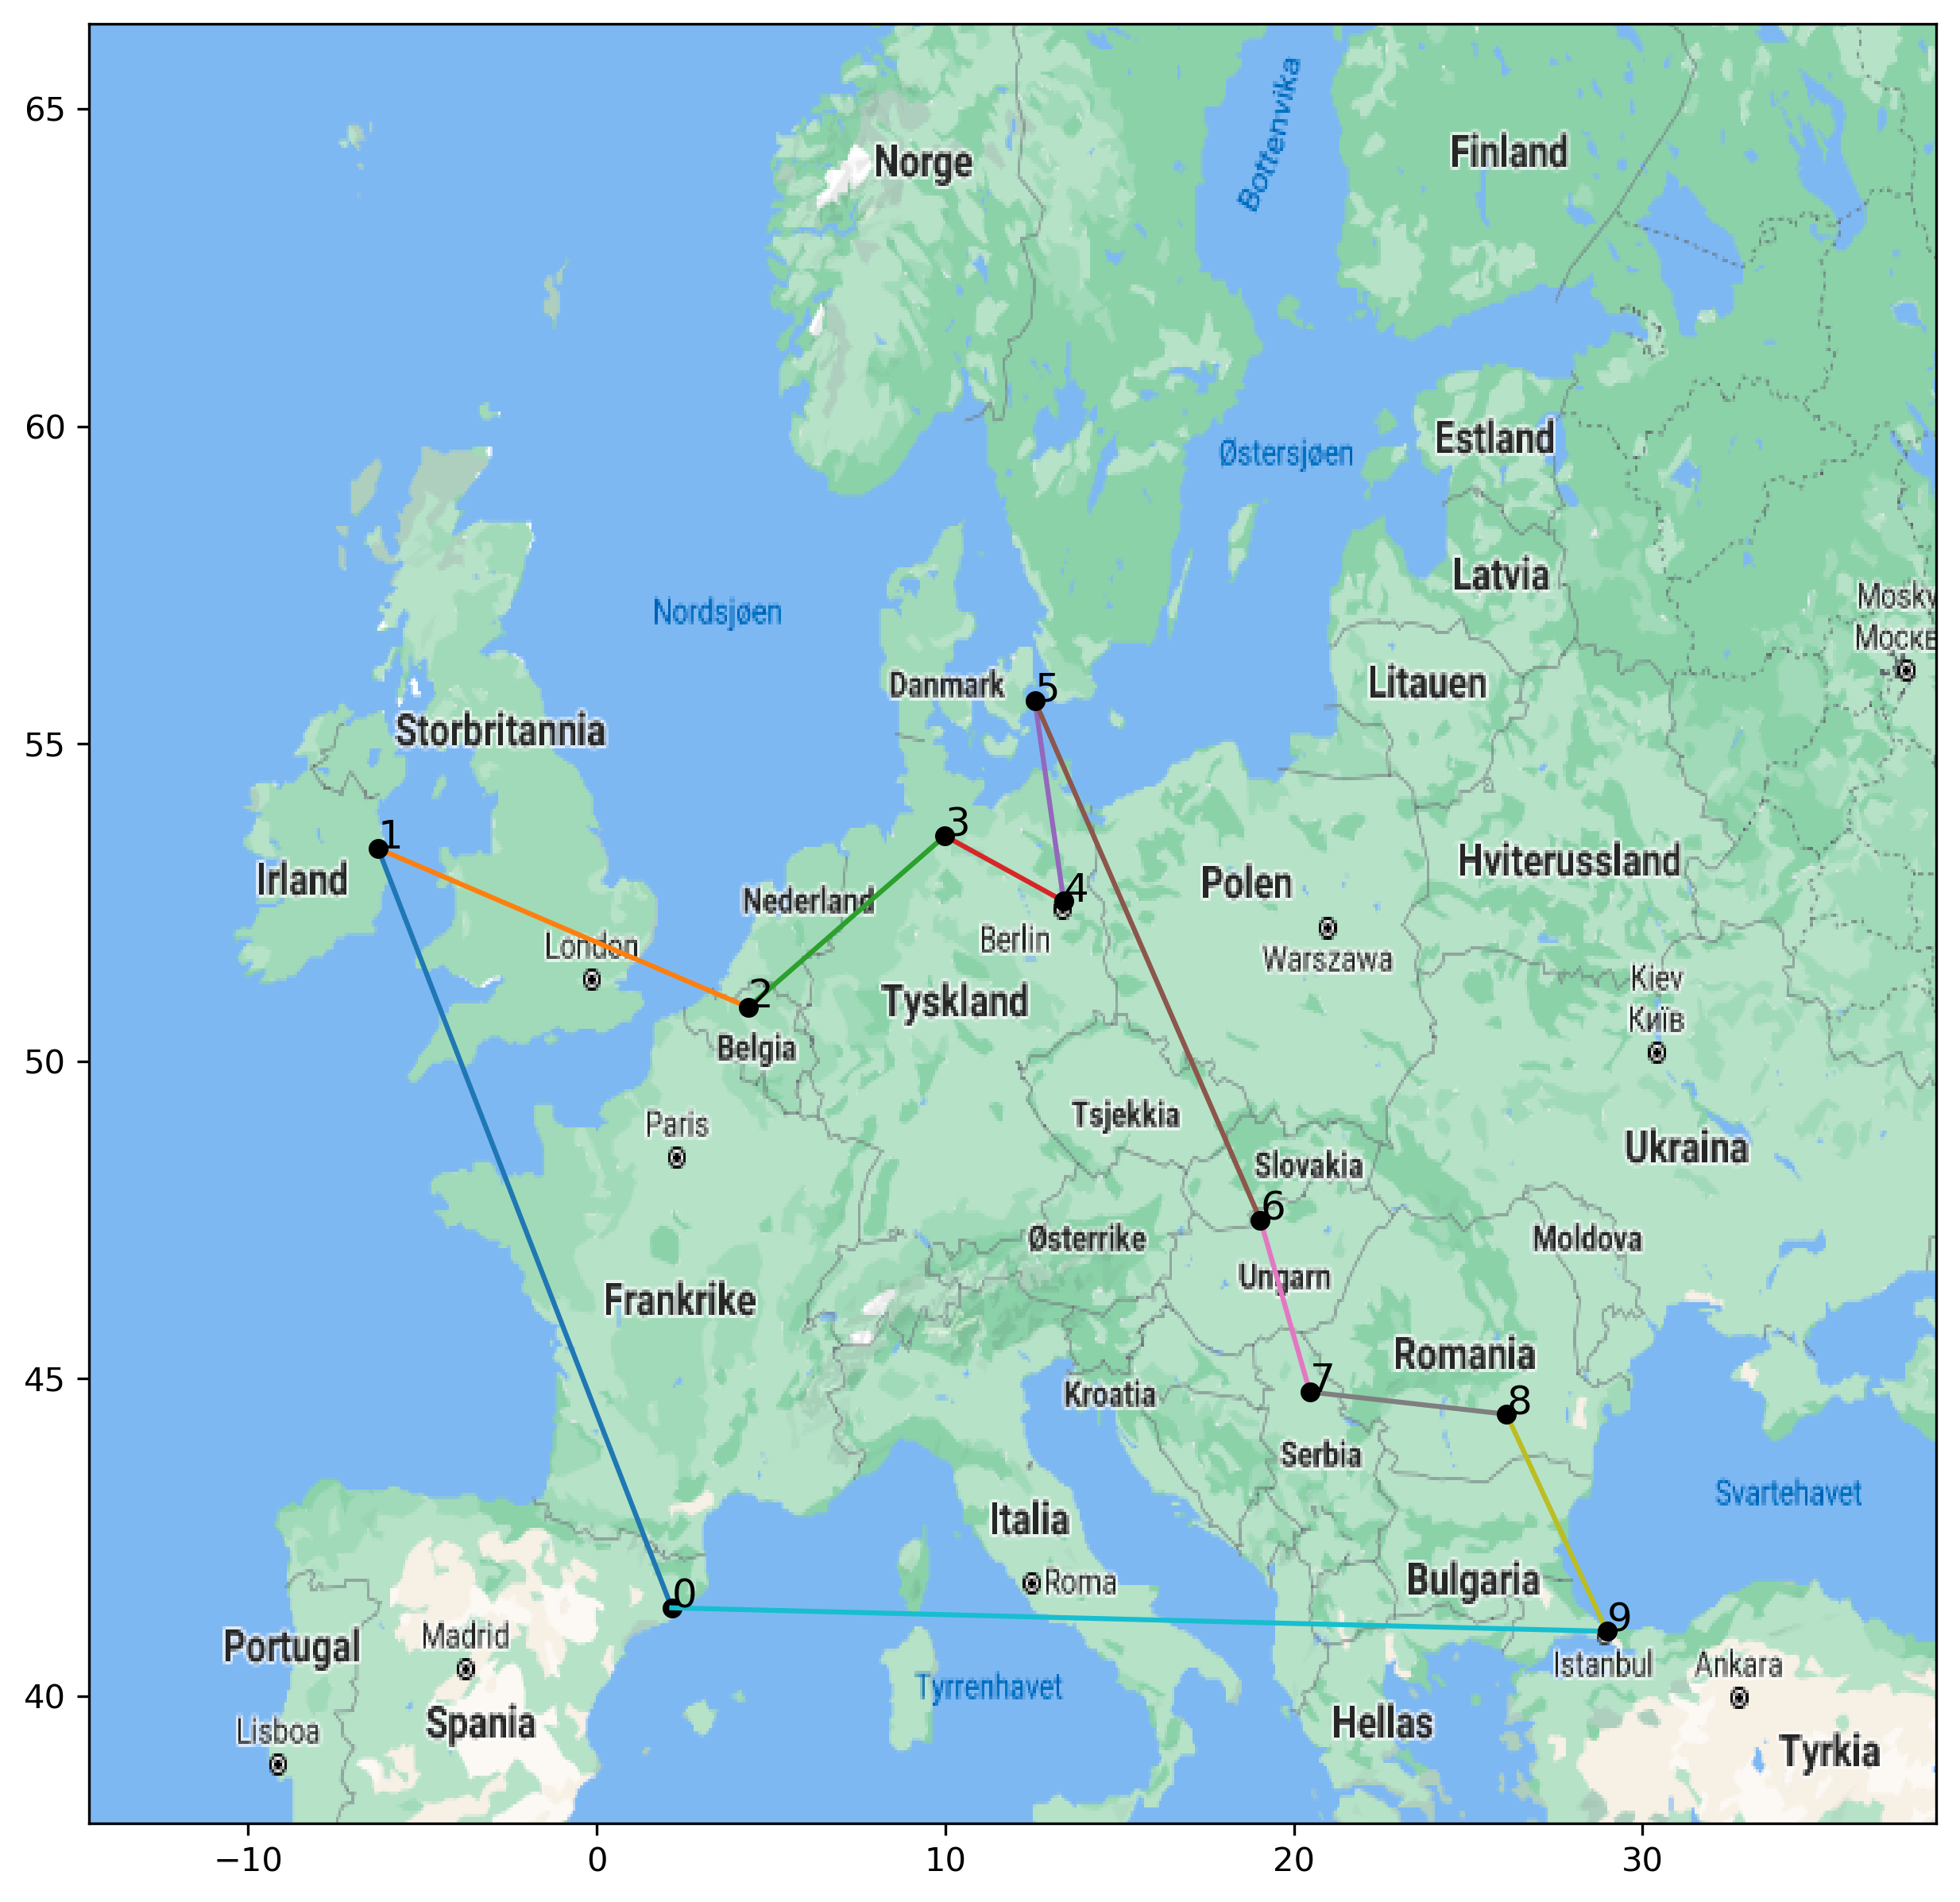
\includegraphics[width=6in, height=4in]{geneticMap3.png}}
\caption{City=10, population=1000, generation=20.}
\label{fig}
\end{figure}
 
\begin{center}
\begin{tabular}{ c c}
 Population & 10  \\ 
 Number of runs & 20  \\ 
 Number of cities & 24  \\  
Tours inspected & 200  \\
 Time used & 0.00798   \\  
 Best run & 21423.9  \\ 
Worst run &  25001.4  \\ 
Average & 23509.9  \\ 
 Standard deviation & 1810.6   \\ 
\end{tabular}
\end{center}


Best sequence of cities: 'Milan', 'Munich', 'Warsaw', 'Dublin', 'Sofia', 'Istanbul', 'Budapest', 'Hamburg', 'Madrid', 'Barcelona', 'Brussels', 'London', 'Paris', 'Copenhagen', 'Stockholm', 'Moscow', 'Saint Petersburg', 'Prague', 'Berlin', 'Rome', 'Belgrade', 'Bucharest', 'Vienna', 'Kiev'\\ 

\begin{figure}[H]
\centerline{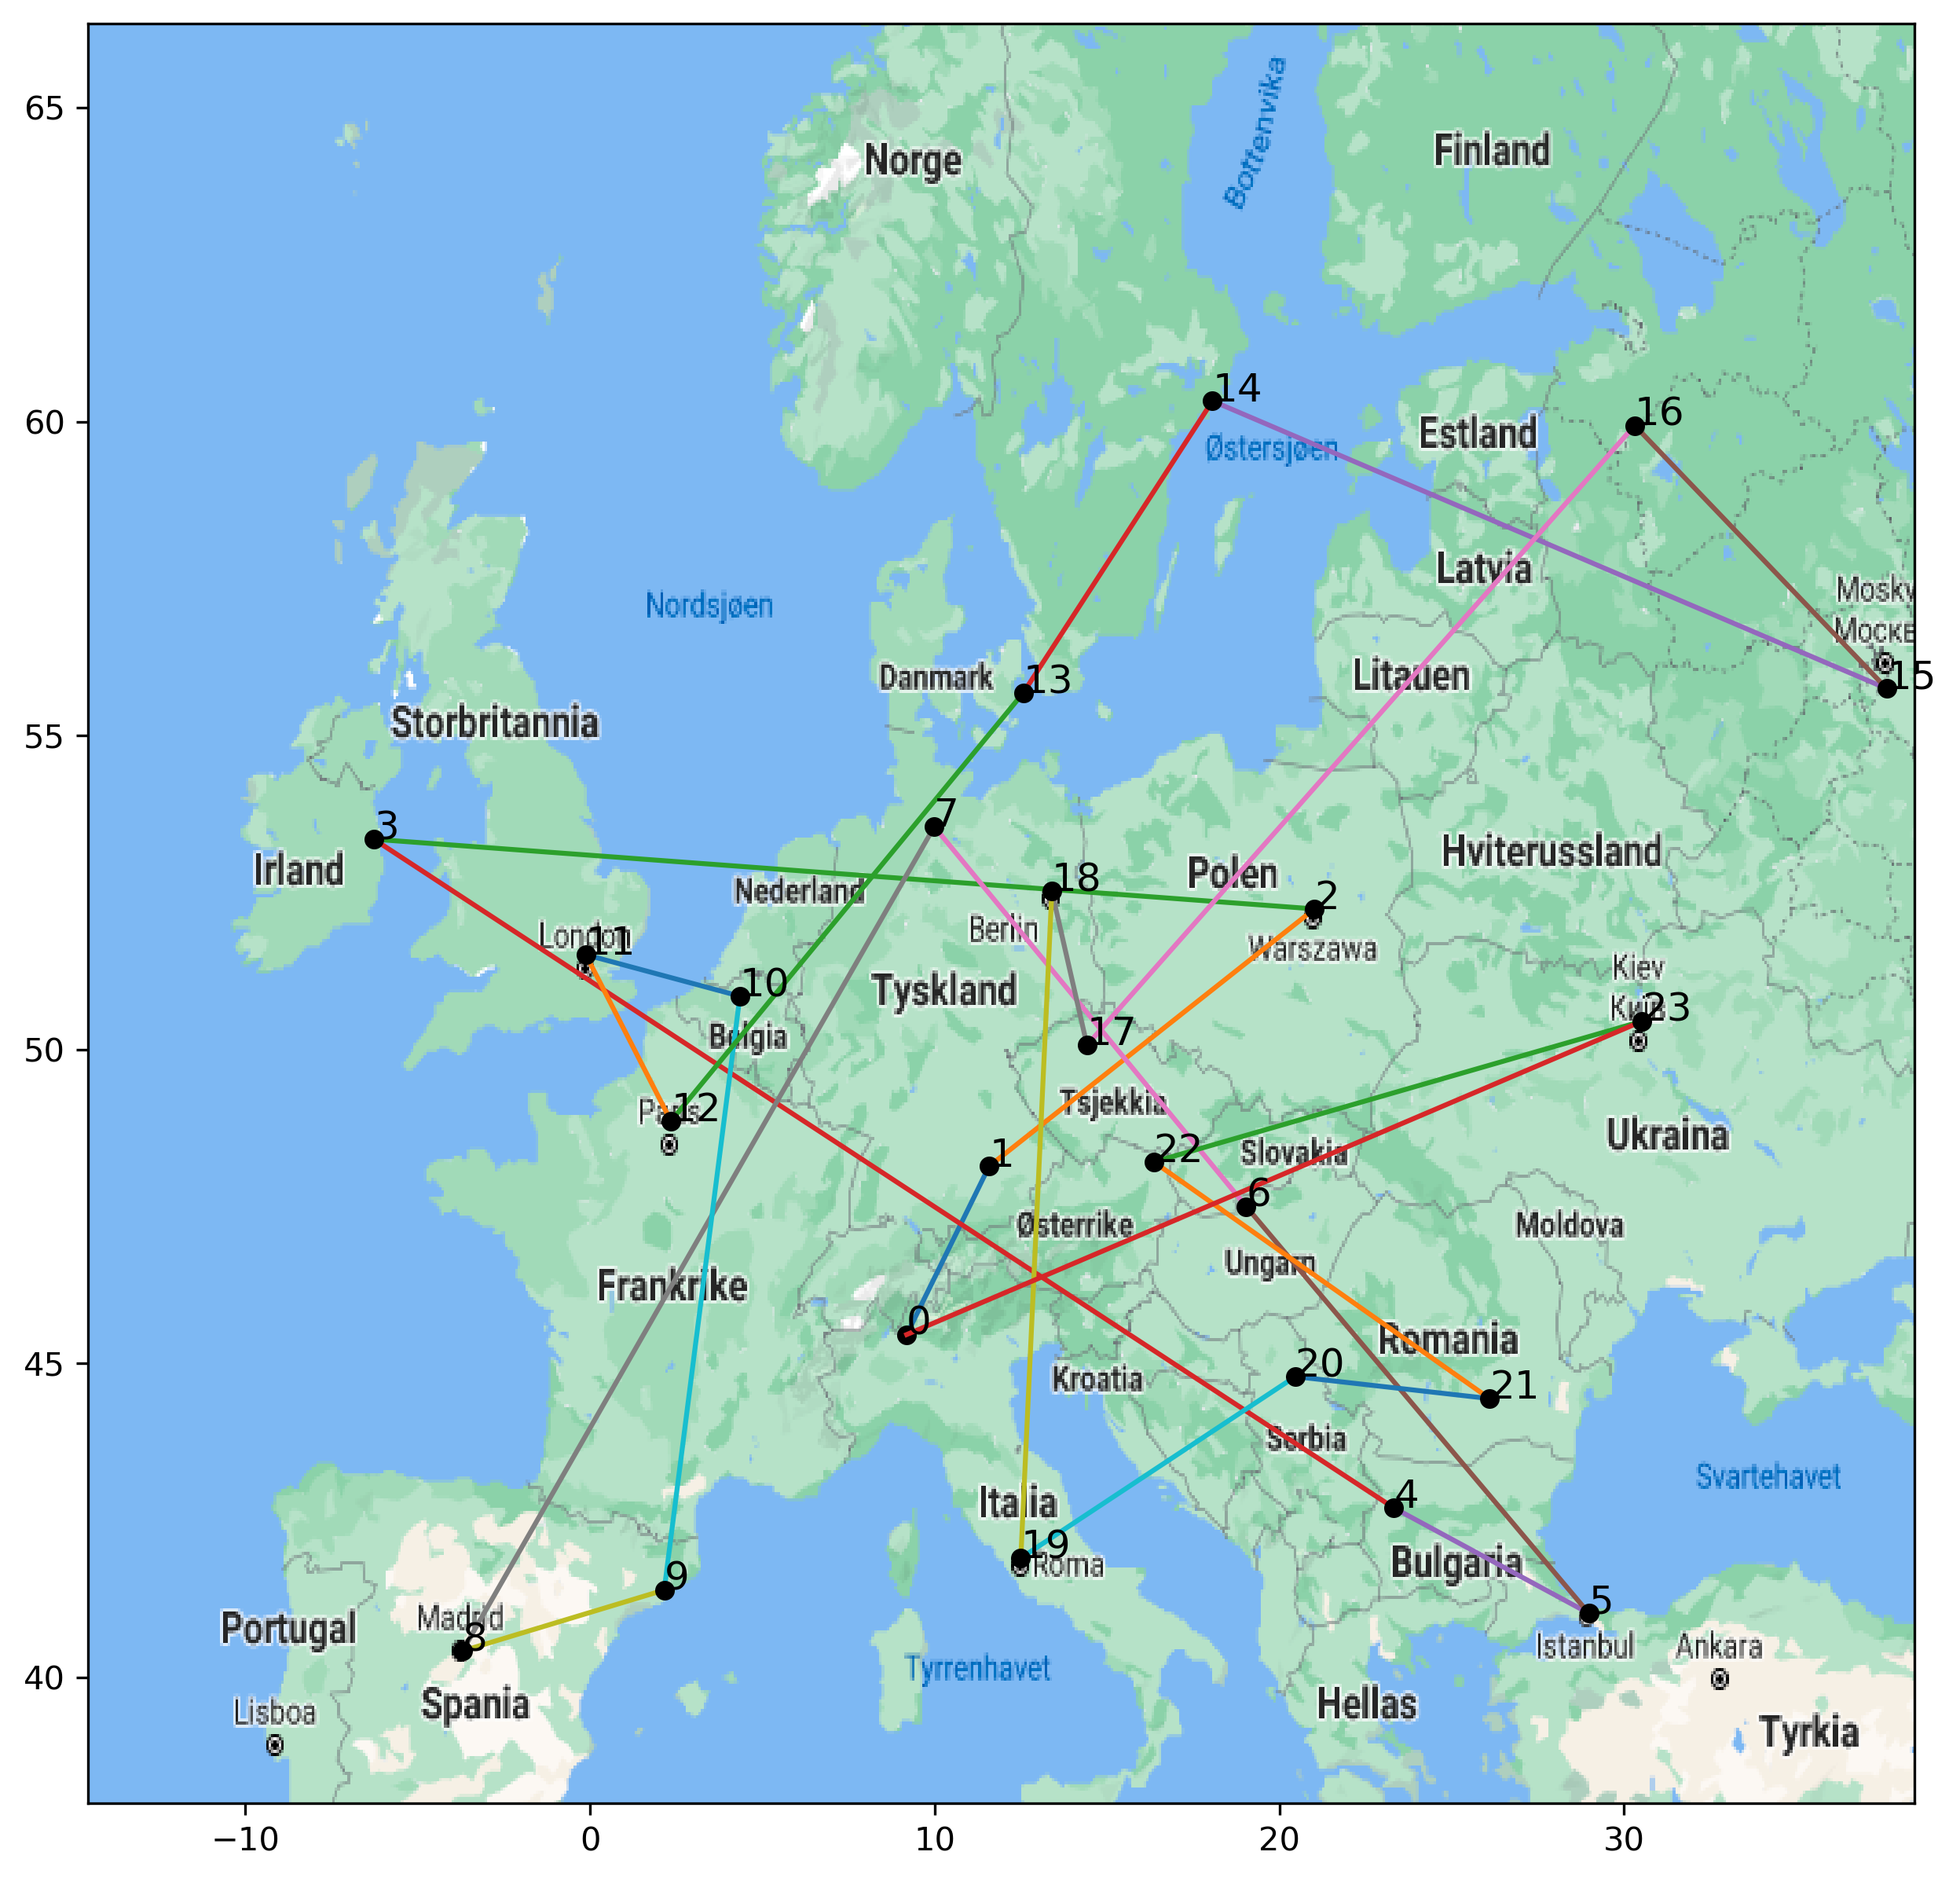
\includegraphics[width=6in, height=4in]{geneticMap4.png}}
\caption{City=24, population=1000, generation=20.}
\label{fig}
\end{figure}

\begin{center}
\begin{tabular}{ c c}
 Population & 100  \\ 
 Number of runs & 20  \\ 
 Number of cities & 24  \\  
Tours inspected & 2000  \\
 Time used & 0.07981   \\  
 Best run & 18717.6  \\ 
Worst run &27158.2  \\ 
Average & 23372.1 \\ 
 Standard deviation & 1698.9   \\ 
\end{tabular}
\end{center}


Best sequence of cities: 'Istanbul', 'Belgrade', 'Moscow', 'Kiev', 'Budapest', 'Sofia', 'Rome', 'Bucharest', 'Hamburg', 'Copenhagen', 'Dublin', 'Brussels', 'London', 'Paris', 'Madrid', 'Barcelona', 'Milan', 'Saint Petersburg', 'Stockholm', 'Berlin', 'Warsaw', 'Munich', 'Prague', 'Vienna'
\begin{figure}[H]
\centerline{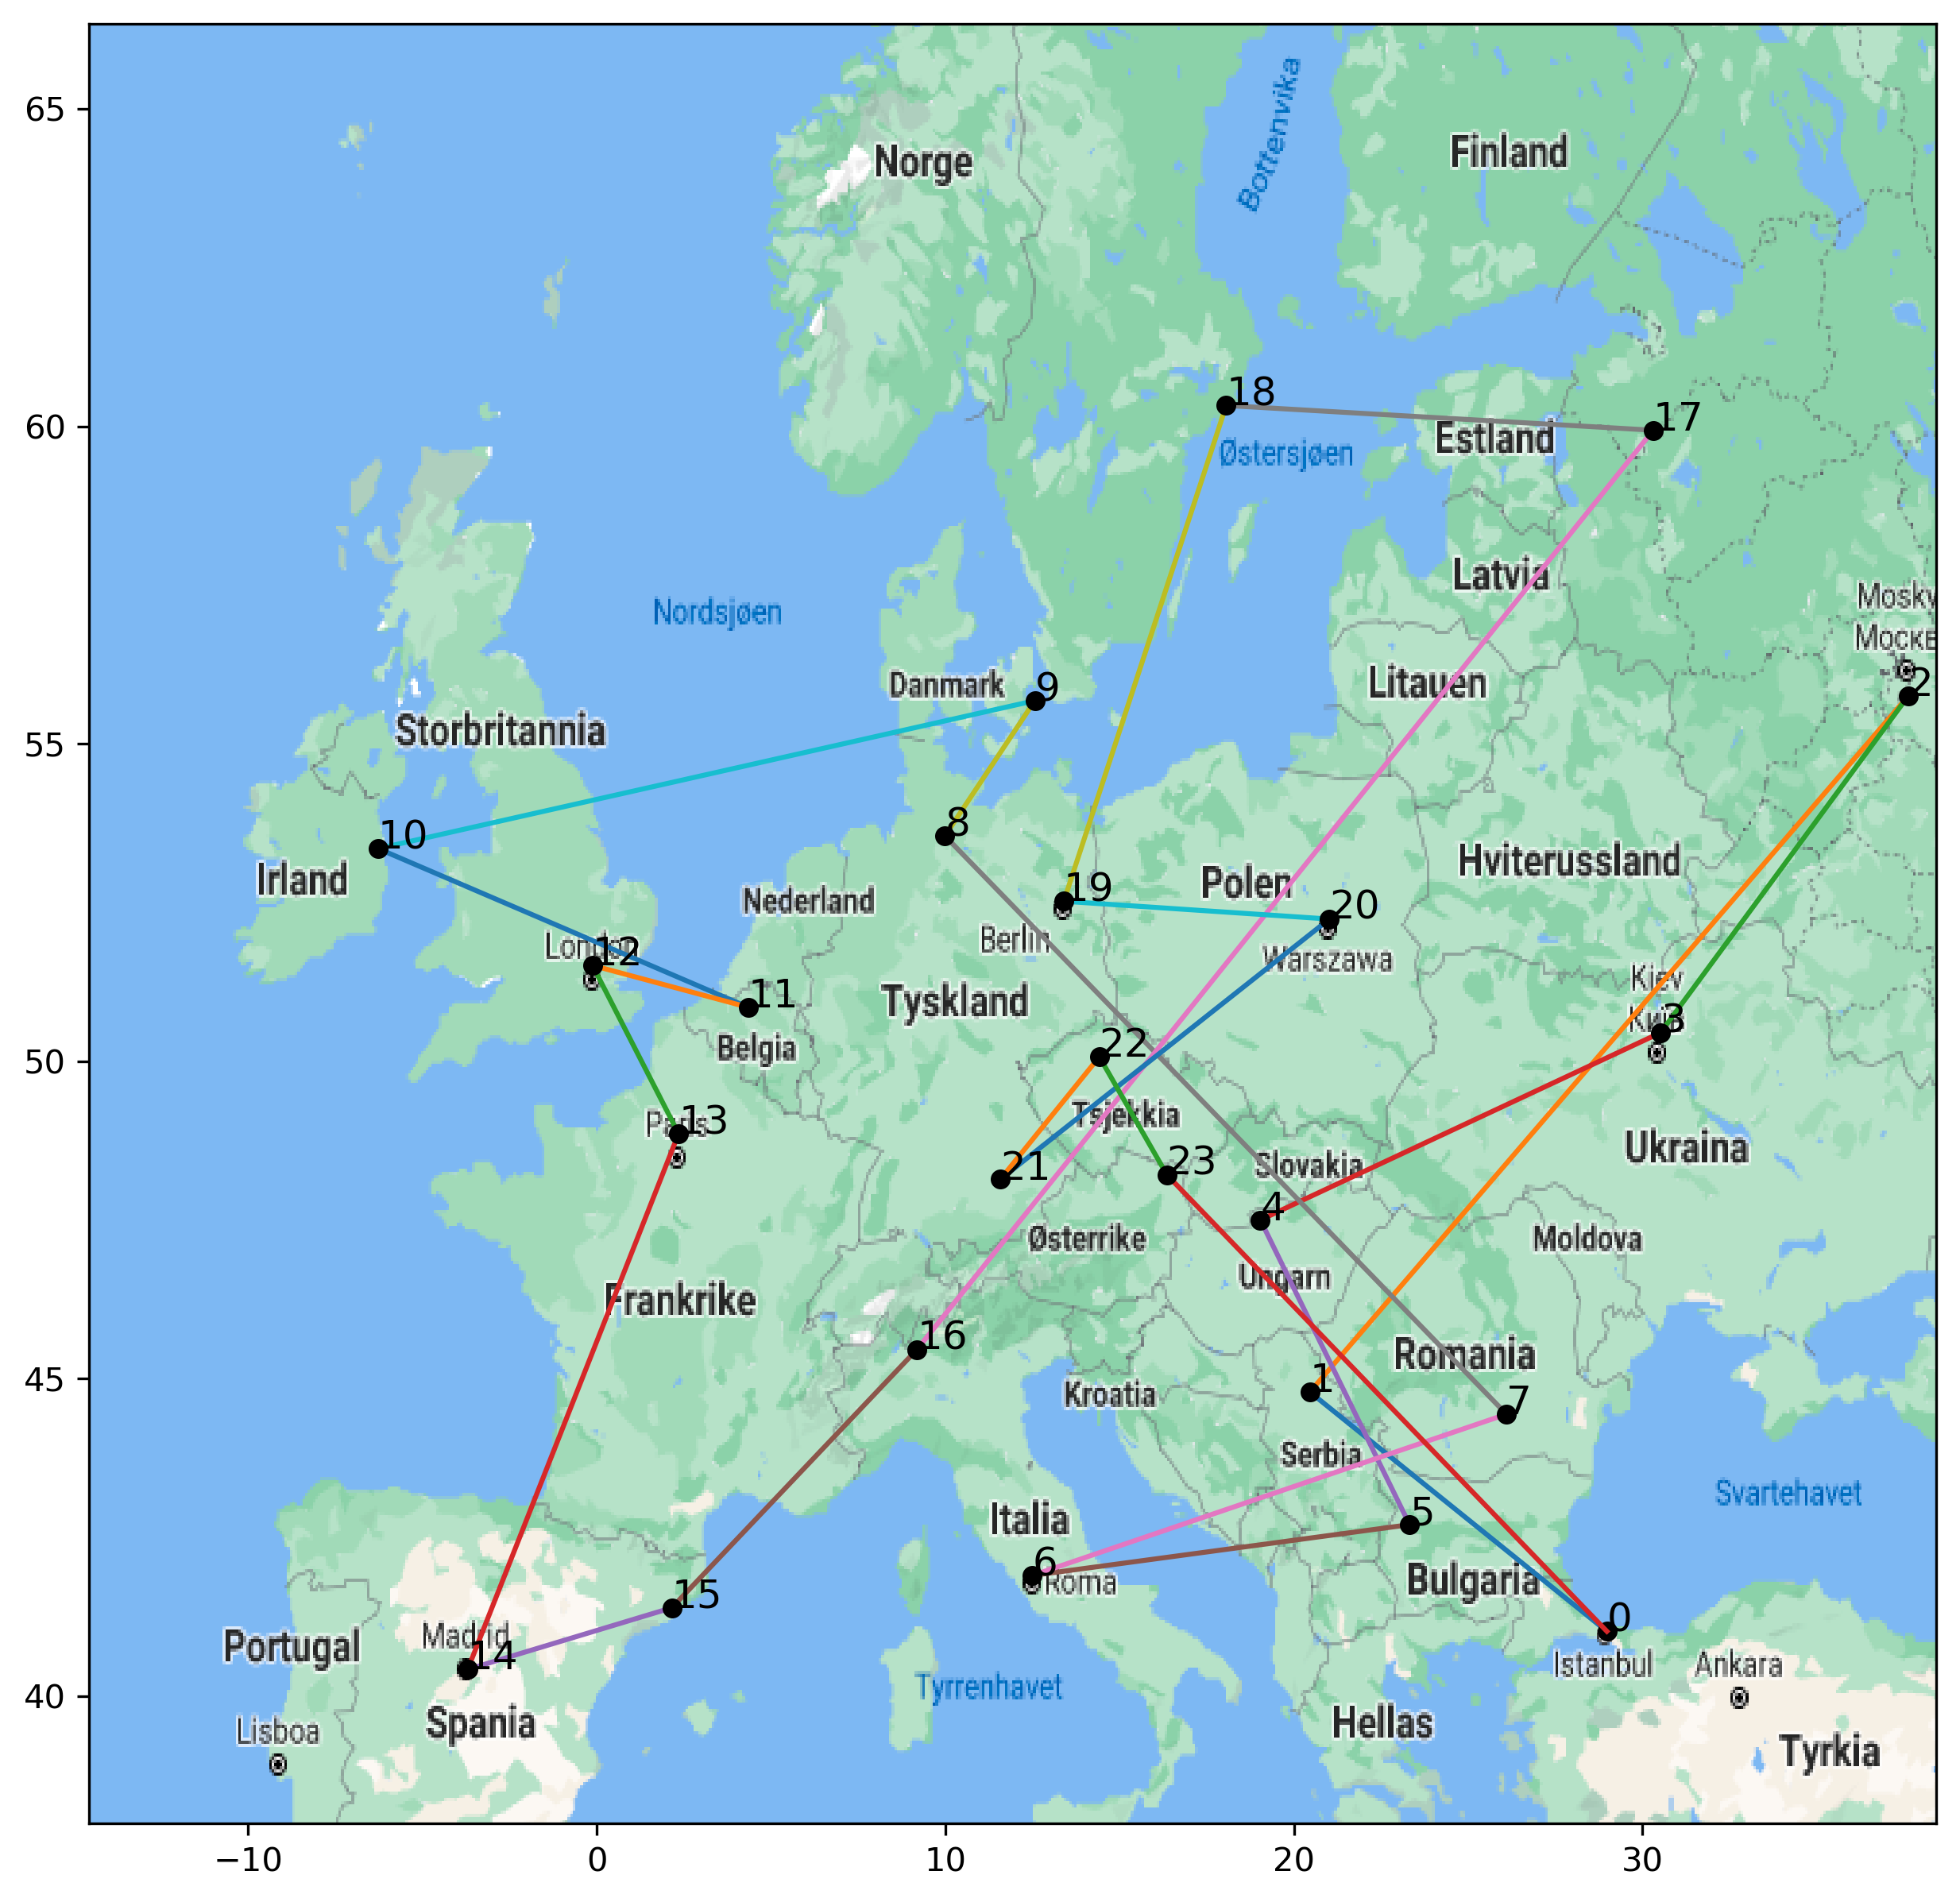
\includegraphics[width=6in, height=4in]{geneticMap5.png}}
\caption{City=24, population=1000, generation=20.}
\label{fig}
\end{figure}

\begin{center}
\begin{tabular}{ c c}
 Population & 1000  \\ 
 Number of runs & 20  \\ 
 Number of cities & 24  \\  
Tours inspected & 20000  \\
 Time used & 0.88566   \\  
 Best run & 17276.0  \\ 
Worst run & 28039.0  \\ 
Average & 23281.4  \\ 
 Standard deviation & 1631.3   \\ 
\end{tabular}
\end{center}


Best sequence of cities: 'Rome', 'Budapest', 'Berlin', 'Kiev', 'Saint Petersburg', 'Moscow', 'Copenhagen', 'Barcelona', 'Madrid', 'Paris', 'Brussels', 'Hamburg', 'Prague', 'Stockholm', 'Munich', 'Vienna', 'Belgrade', 'Bucharest', 'Istanbul', 'Sofia', 'Warsaw', 'Milan', 'London', 'Dublin'

\begin{figure}[H]
\centerline{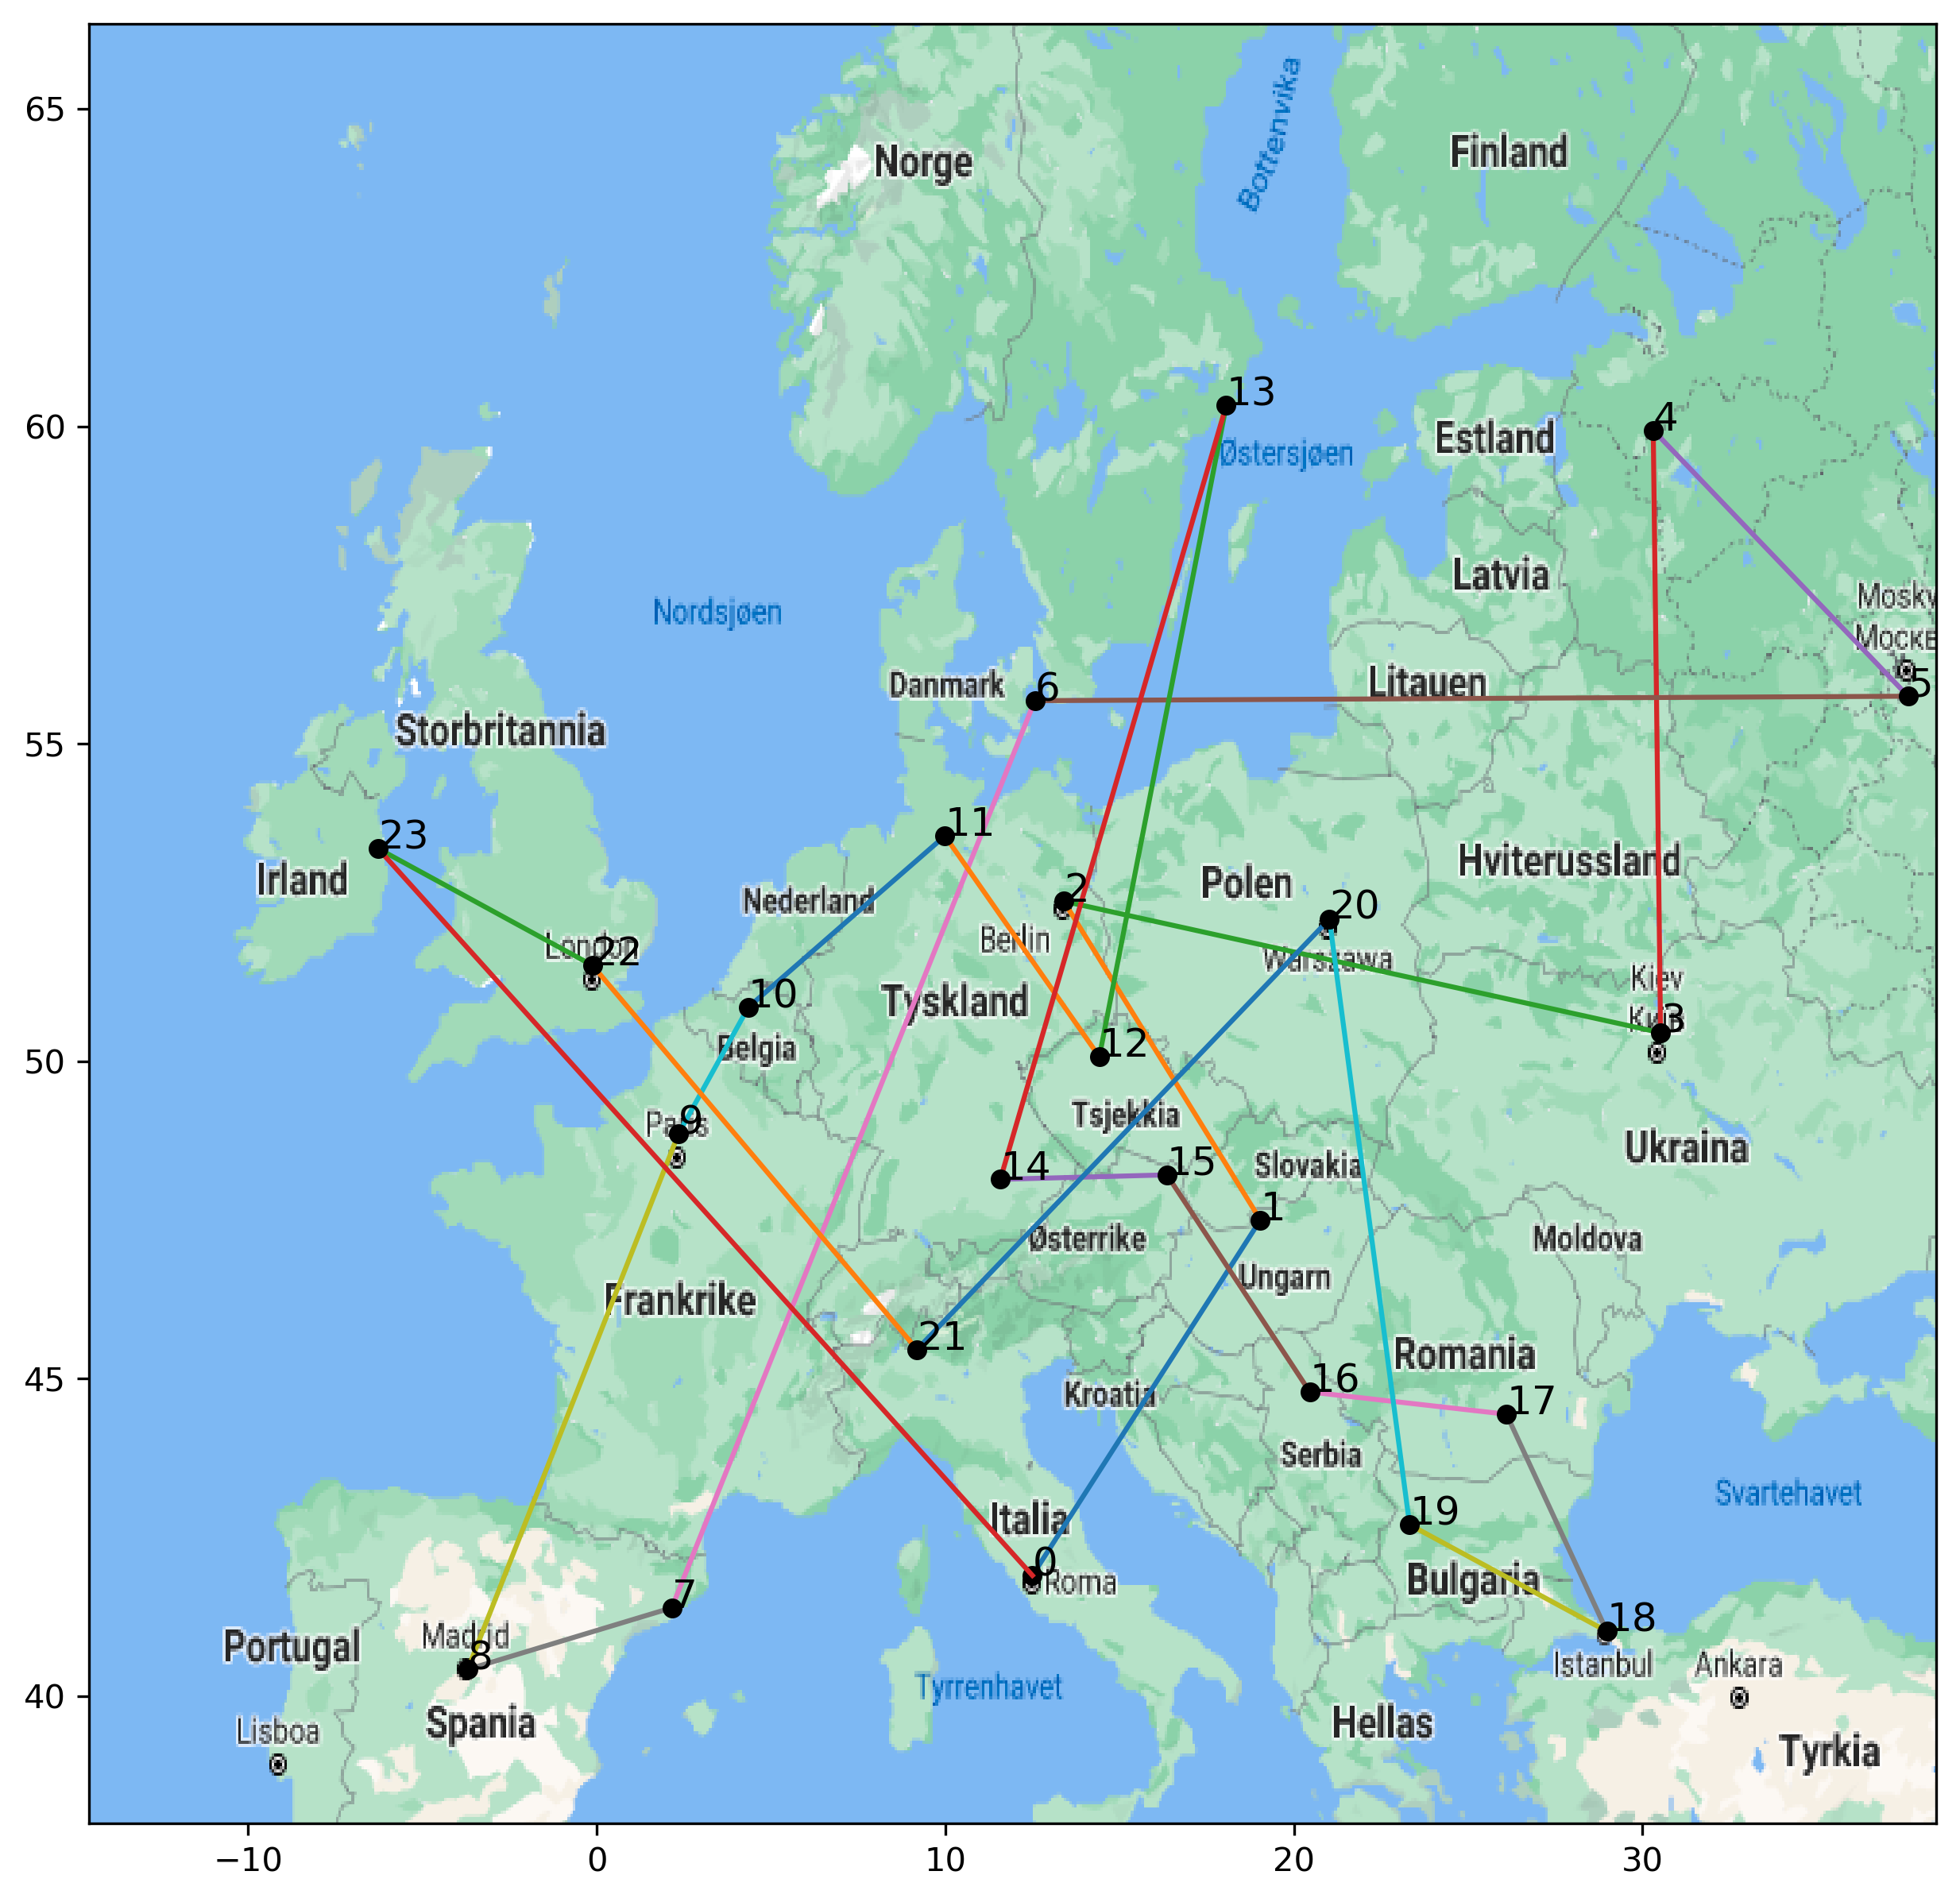
\includegraphics[width=6in, height=4in]{geneticMap6.png}}
\caption{City=24, population=1000, generation=20.}
\label{fig}
\end{figure}
The higher the population, the more exploration and exploitation. This can be seen by looking at the average and the standard deviation values. \\ 

Comparing genetic algorithm and hill climbing for 10 and 24 cities:
\begin{center}
\begin{tabular}{ c c c}
 & GA & HC  \\ 
 Population & 20 & - \\ 
Generations & 200 & - \\ 
 Number of cities & 10 &10  \\  
Tours inspected & 4000 & $10!$ \\
 Time used & 0.075 &  10.001 \\  
 Best run & 5272.7 & 5272.7 \\ 
\end{tabular}
\end{center}

\begin{center}
\begin{tabular}{ c c c}
 & GA & HC  \\ 
 Population & 20 & - \\ 
Generations & 10000 & - \\ 
 Number of cities & 24 & 24 \\  
Tours inspected & 200000 & $24!$ \\
 Time used & 7.786 &  24.75 mill years \\  
 Best run & 10837.1 & 10837.1 \\ 
\end{tabular}
\end{center}

'Dublin', 'London', 'Paris', 'Brussels', 'Hamburg', 'Berlin', 'Warsaw', 'Copenhagen', 'Stockholm', 'Saint Petersburg', 'Moscow', 'Kiev', 'Bucharest', 'Istanbul', 'Sofia', 'Belgrade', 'Budapest', 'Vienna', 'Prague', 'Munich', 'Milan', 'Rome', 'Barcelona', 'Madrid'

\begin{figure}[H]
\centerline{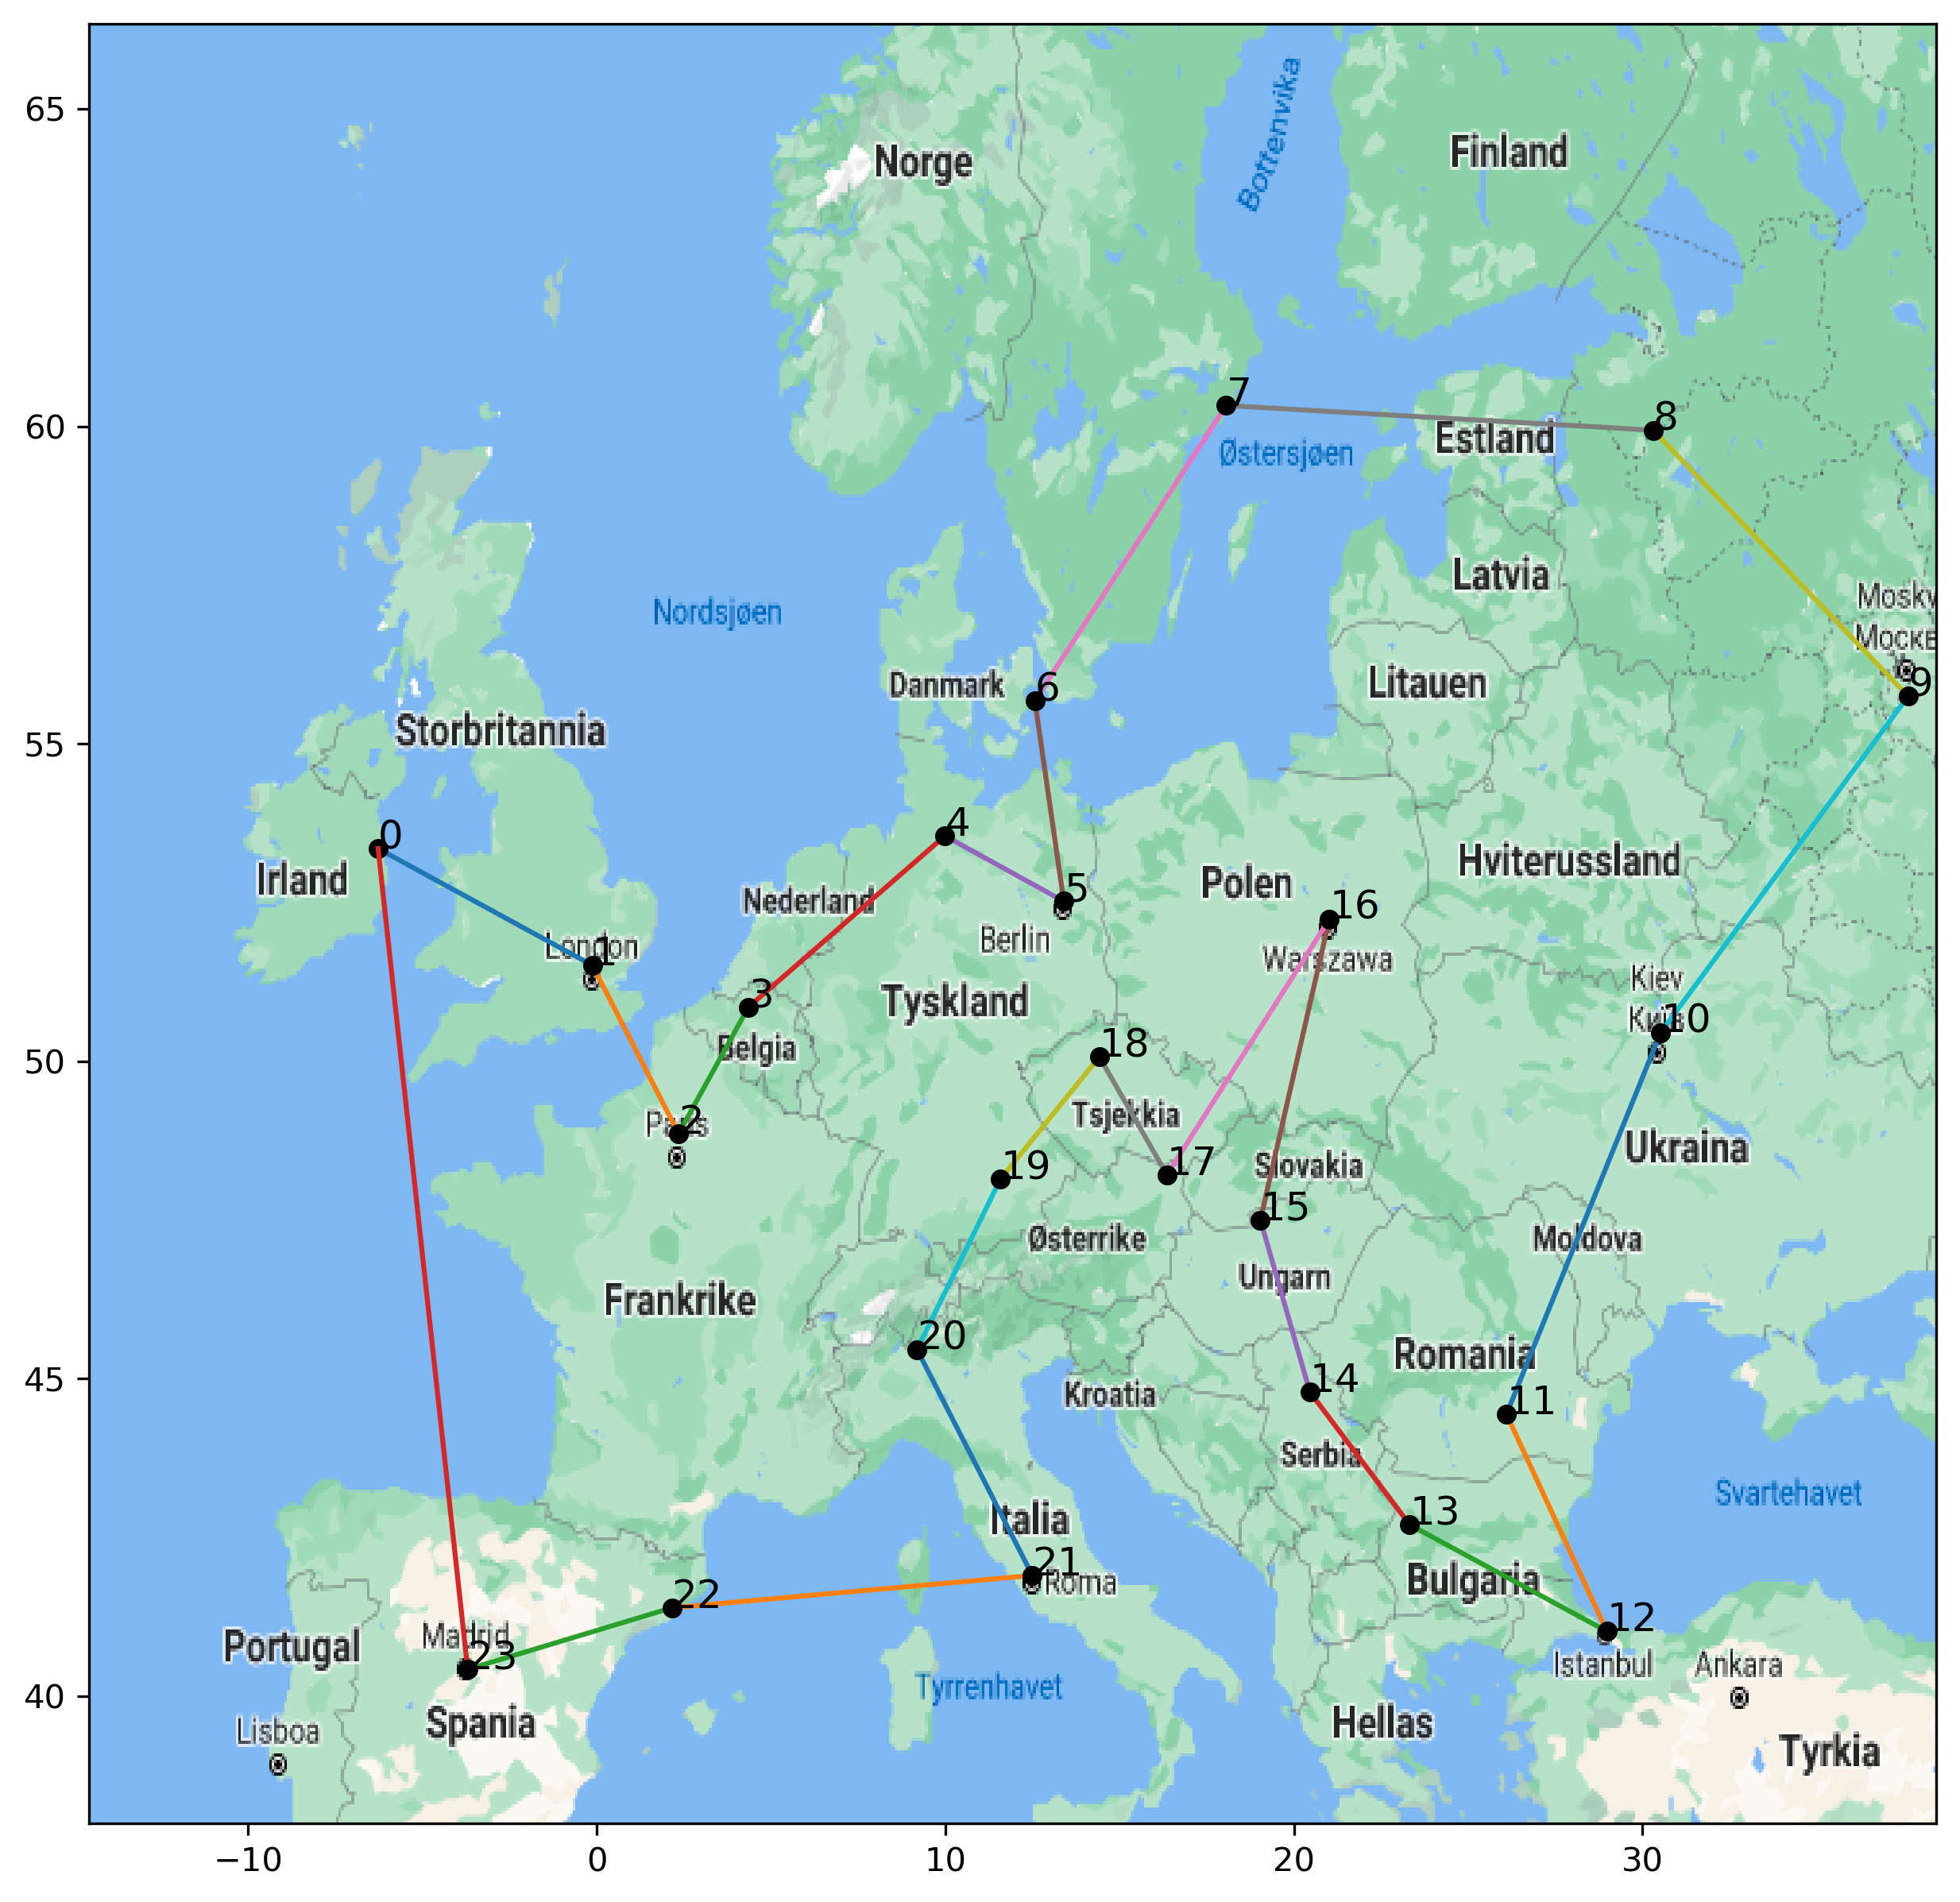
\includegraphics[width=6in, height=4in]{geneticMap7.png}}
\caption{City=24, population=20, generation=10000.}
\label{fig}
\end{figure}

\begin{figure}[H]
\centerline{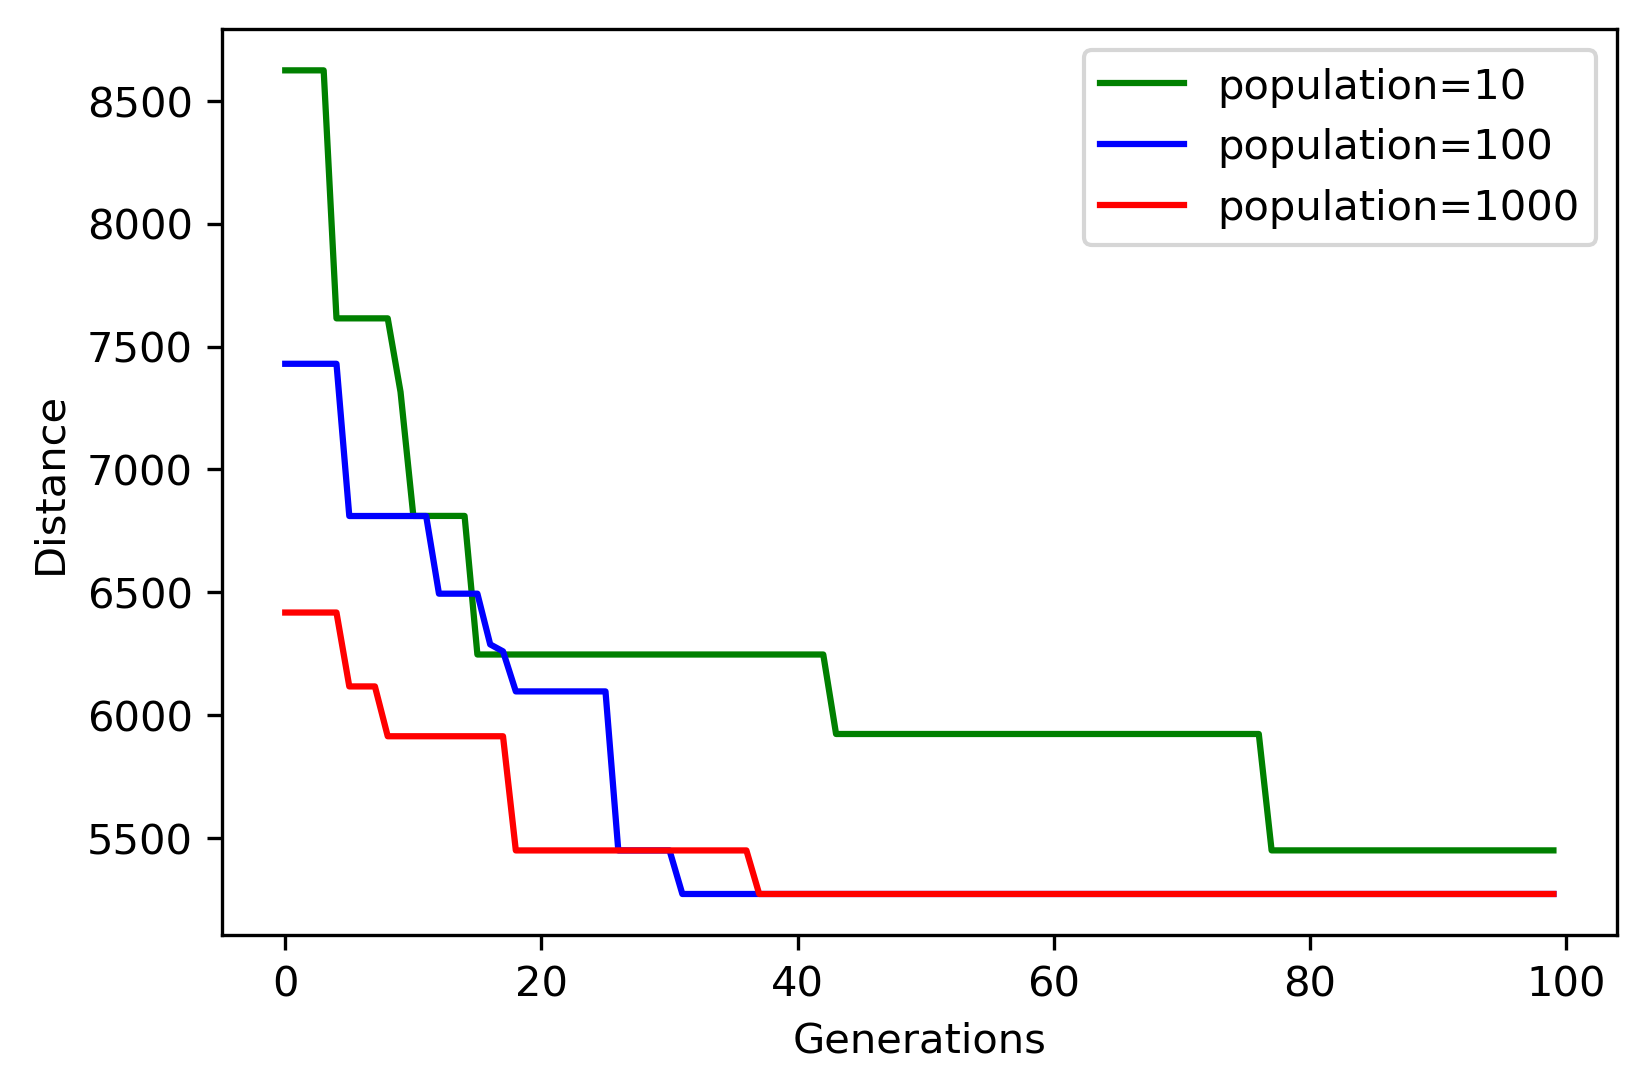
\includegraphics[width=6in, height=4in]{genetic.png}}
\caption{3 different populations for 10 cities}
\label{fig}
\end{figure}

\begin{figure}[H]
\centerline{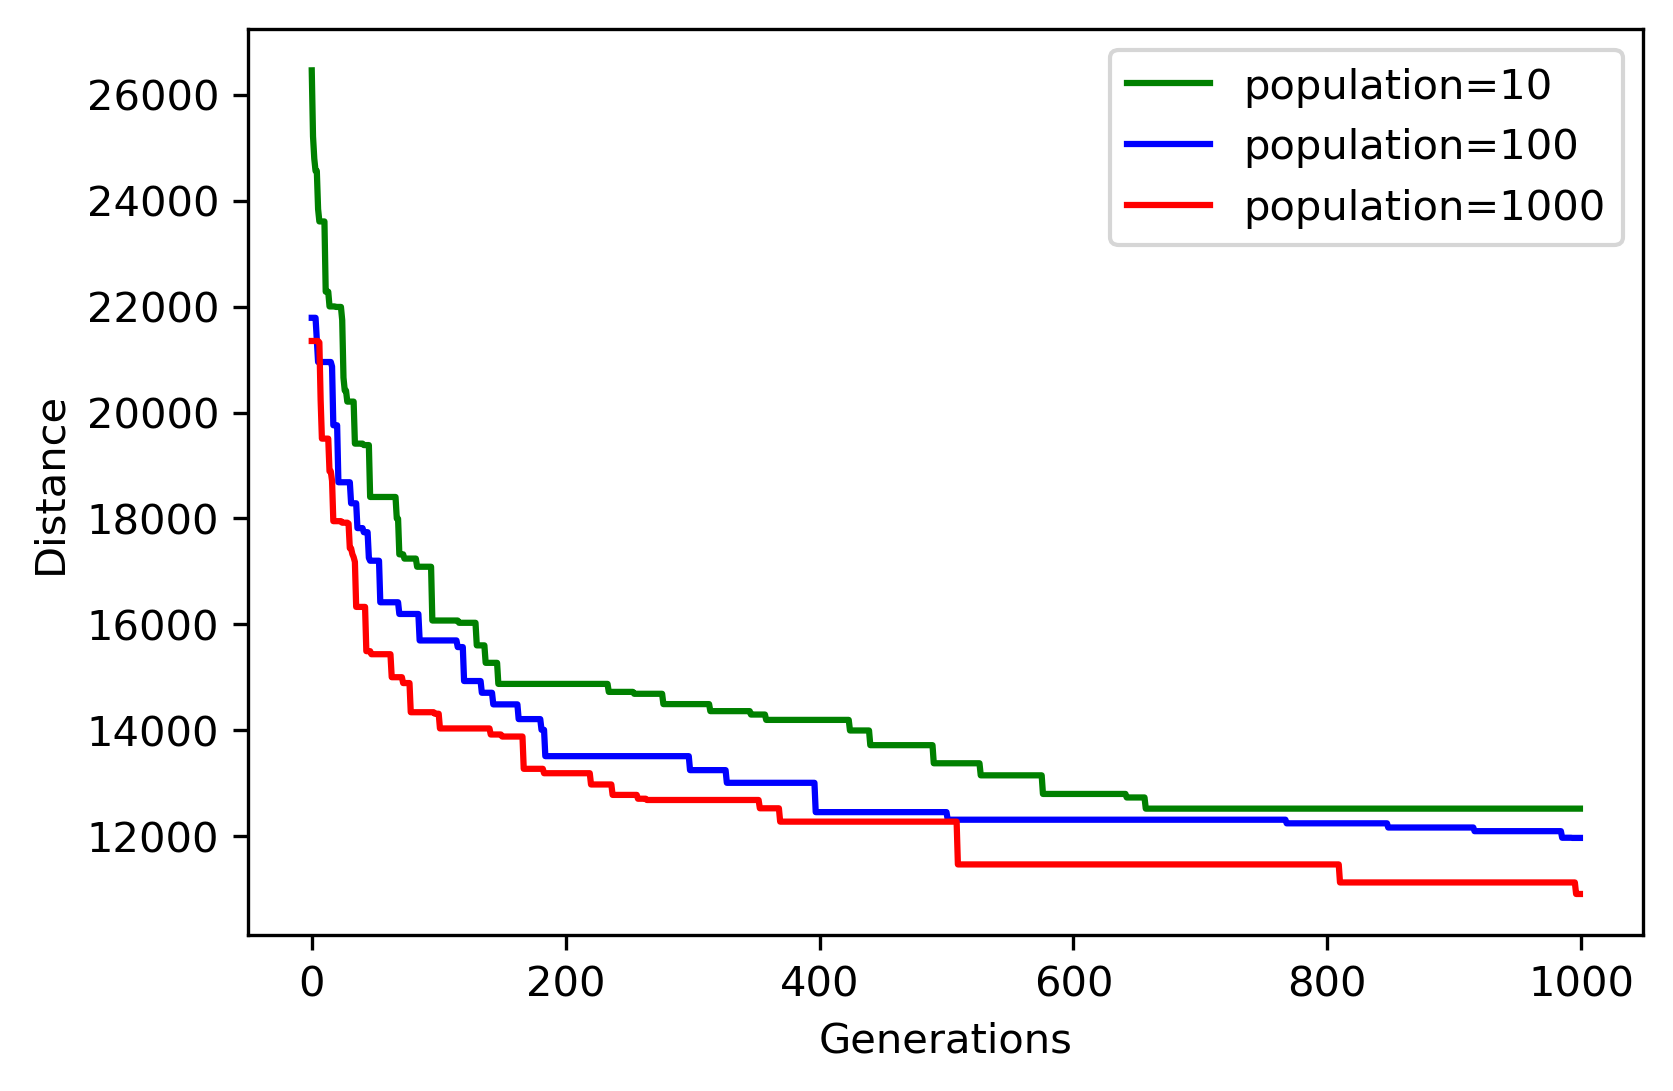
\includegraphics[width=6in, height=4in]{genetic1.png}}
\caption{3 different populations for 24 cities}
\label{fig}
\end{figure}

From the tables and graph we can see that the bigger population size the smaller generations it takes to find a global min, however this is will take a lot longer. It is therefore more efficient to use small population and bigger generations.

\section{Hybrid genetic algorithm}
Hybrid genetic algorithm is a mix of genetic algorithm and hill climbing. In the Baldwinian algorithm we start by running the Hill climber for 10 $\%$ of random parents and in each population and 2 random genes are swapped.This is repeated 10 times, and the parent with best mutation will be chosen to through mutation and recombination. In the Lamarckian algorithm the best mutated individual will be chosen in the population. After this, we run the genetic algorithm and compare the two GA variants.

\begin{center}
\begin{tabular}{ c c c c}
& Baldwinian & Lamarckian \\ 
Number of cities & 10 &10\\ 
Generations & 100 &100\\ 
Population & 100&100 \\  
Routes    &1001000 &1001000 \\
 time (s) &  5.77 & 5.98\\  
 Best distance & 5272.68 & 5272.68 \\ 
 Worst distance & 5673.40 & 5959.90 \\ 
 Average distance  & 5371.44 & 5341.03 \\ 
 Standard deviation  & 119.91 &118.78 
\end{tabular}
\end{center}


\begin{figure}[H]
\centerline{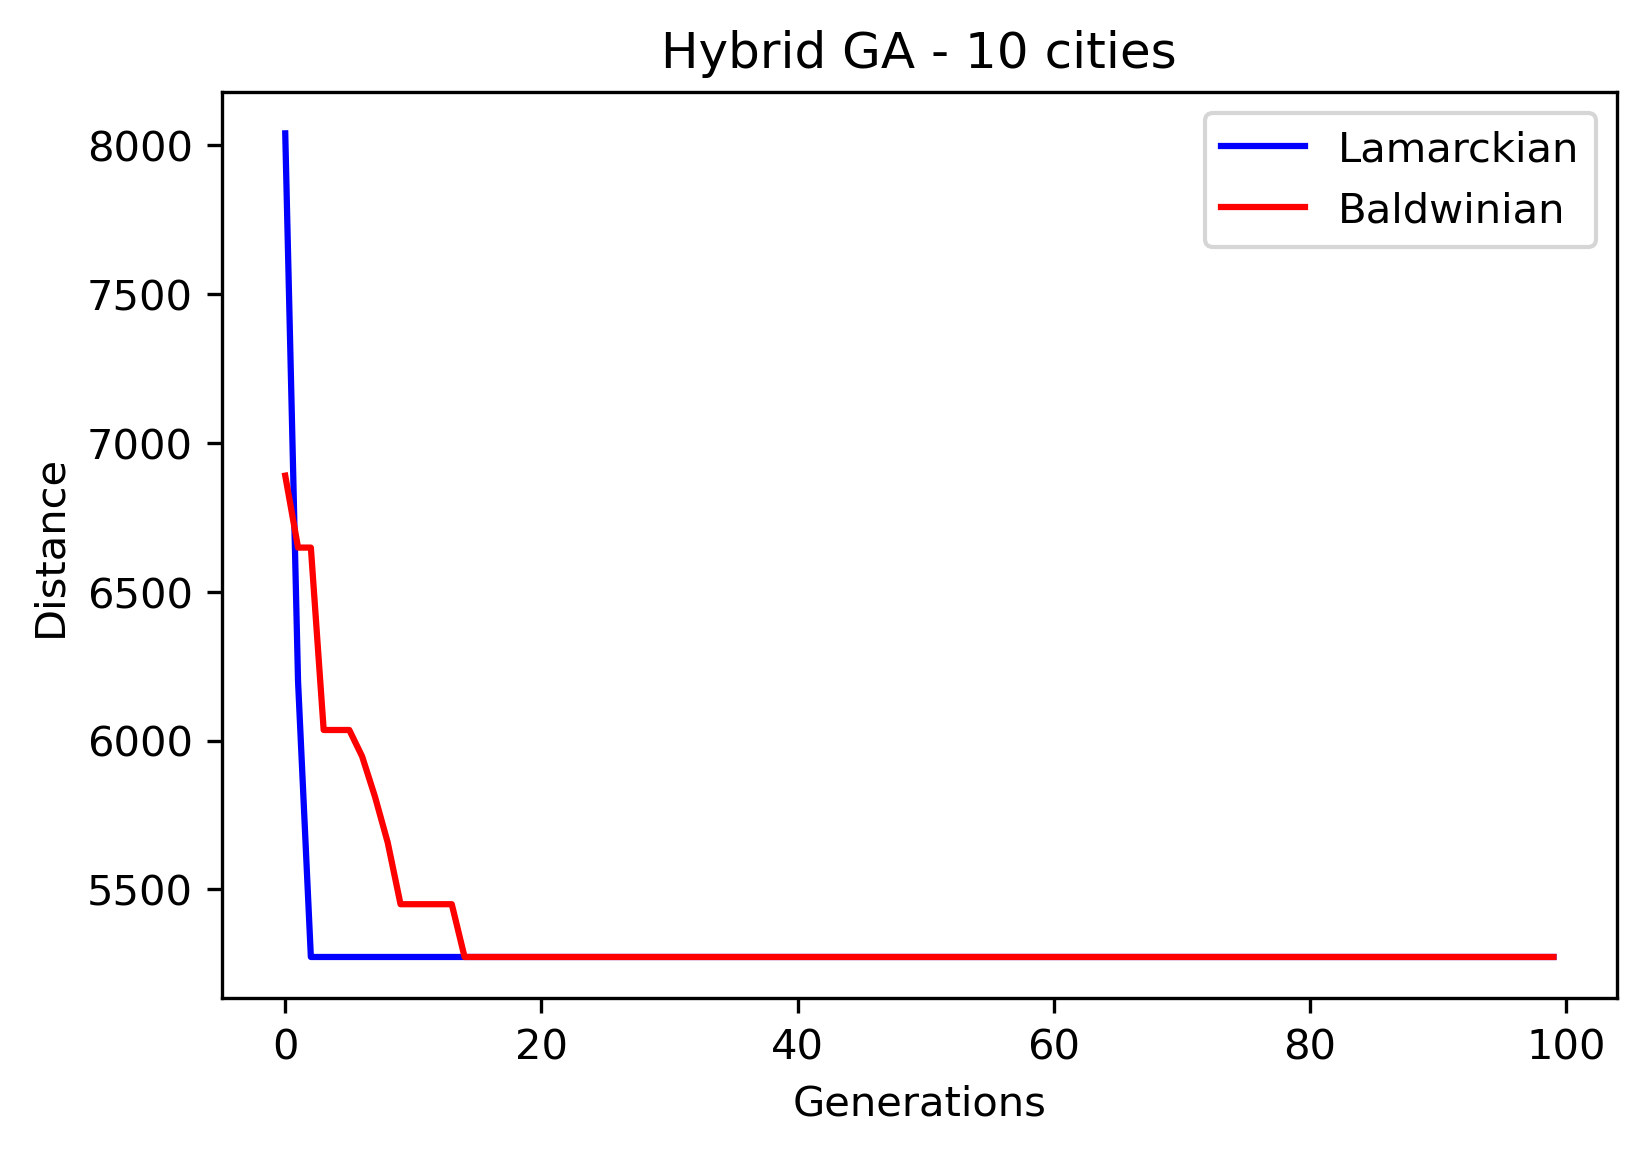
\includegraphics[width=6in, height=4in]{hybridGen10.png}}
\caption{Comparing the two algorithms.}
\label{fig}
\end{figure}

\begin{center}
\begin{tabular}{ c c c c}
& Baldwinian & Lamarckian \\ 
Number of cities & 24 &24\\ 
Generations & 100 &100\\ 
Population & 100&100 \\  
Routes    &1001000 &1001000 \\
 time (s) &  9.90 & 10.05\\  
 Best distance & 12007.99 & 11252.31 \\ 
 Worst distance & 14221.46 & 13608.77 \\ 
 Average distance  & 13015.62 & 12270.63 \\ 
 Standard deviation  & 484.30 & 493.67 
\end{tabular}
\end{center}

\begin{figure}[H]
\centerline{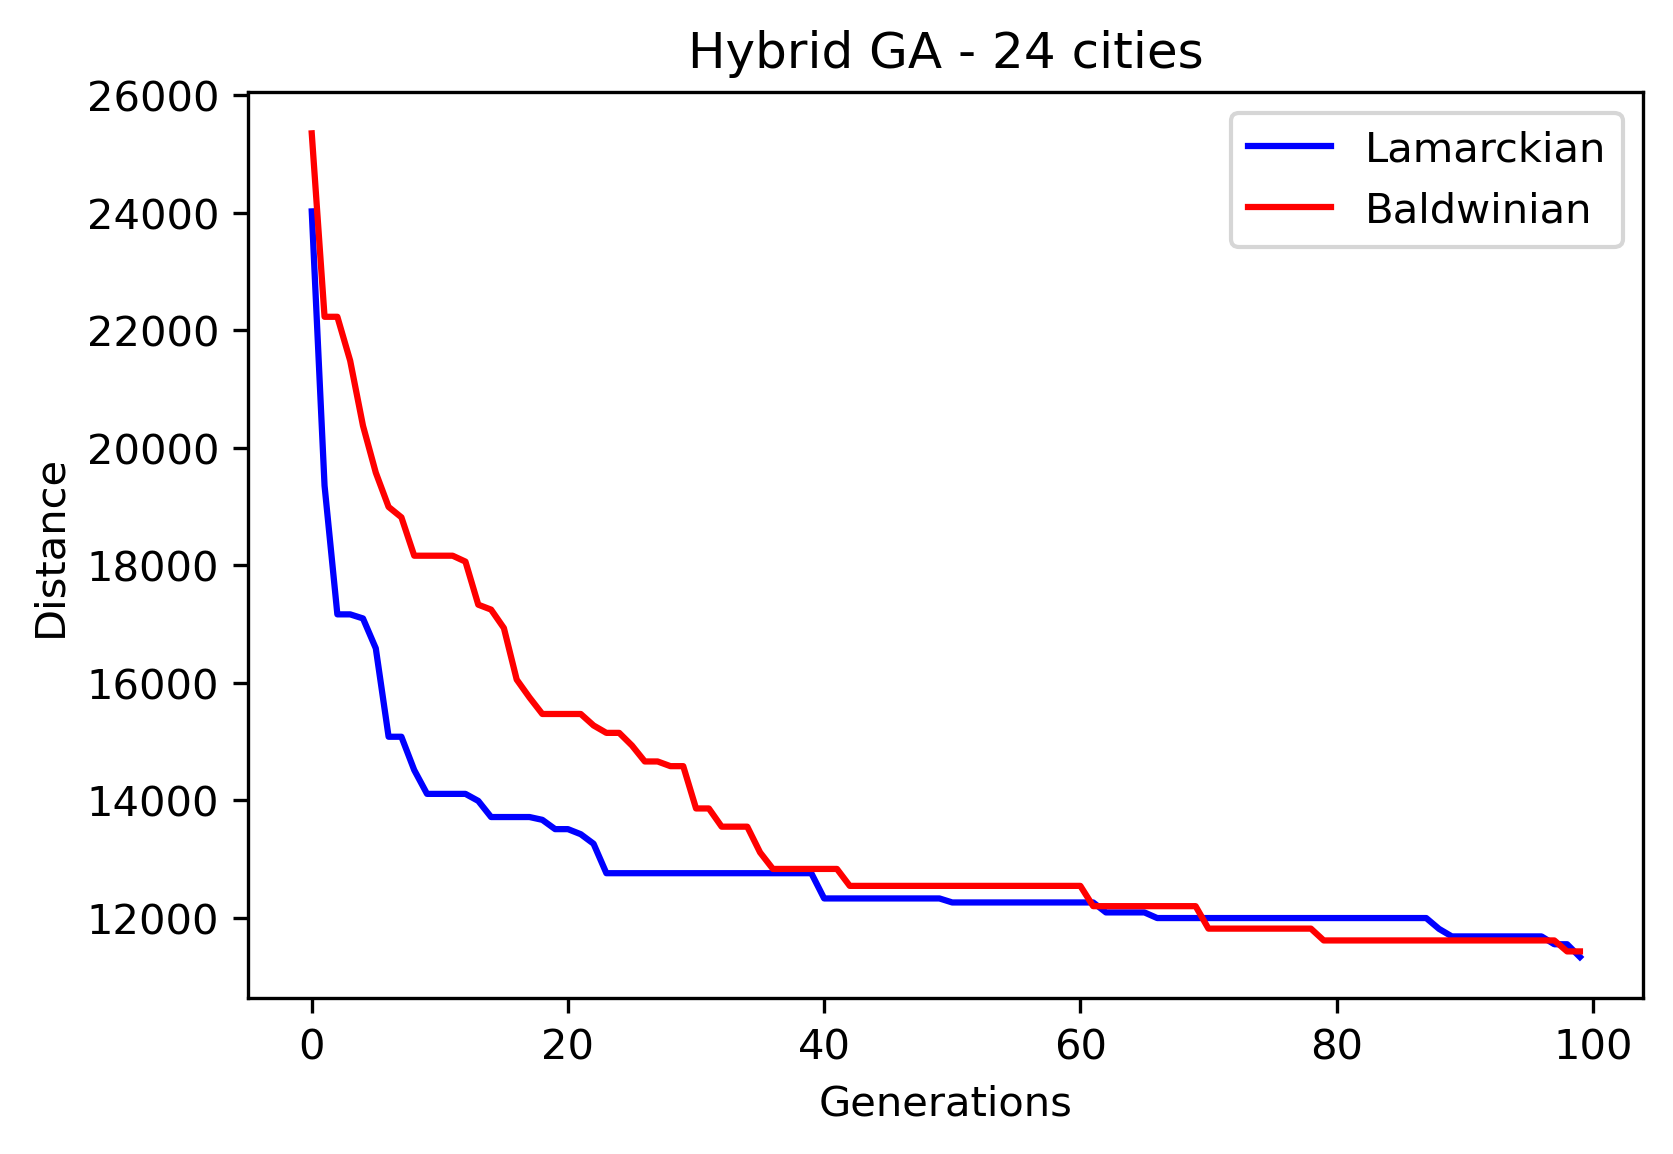
\includegraphics[width=6in, height=4in]{hybridGen20.png}}
\caption{Comparing the two algorithms.}
\label{fig}
\end{figure}

From the tables and graph in this section, we can see that Lamarckian algorithm finds the best solution with least generations. Baldwinian also provides good solutions. This is actually not always the case, Lamarckian and Baldwinian algorithms alternate. Sometimes the Baldwinian provides a better solution. Comparing the two to pure GA, there is a big diffrence. The hybrid version find a solution with much lower iterations, however this comes at cost of time. The time it takes to find a global solution using hybrid GA is much slower that of pure GA. 




\end{document}